%%  export TEXINPUTS=.:/home/mjw/src/manuals/common:

\documentclass[11pt,a4paper,openany,oneside]{book}

\usepackage[usenames]{color}
\usepackage{dirtree}
\usepackage{epsfig}
\usepackage{fancyhdr}
\usepackage{listings}
\usepackage{graphicx}
\usepackage{parskip}
\usepackage{pifont}
\usepackage{rotating}
\usepackage{enumitem}
\usepackage{latexsym}
\usepackage{titlesec}
\usepackage{xcolor}
\usepackage{fancybox}
\usepackage{caption}
\usepackage{subcaption}
\usepackage{hyperref} % wants to be last

\hypersetup{
  colorlinks   = true, %Colours links instead of ugly boxes
  urlcolor     = blue, %Colour for external hyperlinks
  linkcolor    = blue, %Colour of internal links
  citecolor   = red %Colour of citations
}

\pagestyle{fancy}
\renewcommand{\chaptermark}[1]{\markboth{\thechapter.\ #1}{}} 
\fancyhead[LE,LO]{\slshape \leftmark}
\fancyhead[RE,RO]{}

% Define some colours
\definecolor{OTTPGreen}{rgb}{0,0.341,0}

% Set formats for each heading level

\titleformat{\chapter}
{}
{\Huge\bfseries\sffamily\color{OTTPGreen}  \thechapter .\space}
{0pt}
{\Huge\bfseries\sffamily\color{OTTPGreen}}

% Change the format of sections
\titleformat*{\section}{\Large\bfseries\sffamily\color{OTTPGreen}}
\titleformat*{\subsection}{\large\bfseries\sffamily\color{OTTPGreen}}
\titleformat*{\subsubsection}{\normalsize\bfseries\sffamily\color{OTTPGreen}}

\newcommand{\ci}[1]{\hspace*{1cm} {\small\texttt{#1}}}
\newcommand{\cc}[1]{{\texttt{#1}}}
\newcommand{\mykey}[1]{{\makebox[16pt] {\put(0,4){\circle{12}} \put(0,4){\makebox(0,0){\small{#1}}}}}}

\newcommand{\sysname}{{TTP}}
\newcommand{\longsysname}{{Time Transfer Platform}}

% Set bullet style
\renewcommand{\labelitemi}{$\Box$} 
\renewcommand{\labelitemii}{$\Box$} 
\renewcommand{\labelitemiii}{$\Box$} 
\renewcommand{\labelitemiv}{$\Box$} 

\newenvironment{description*}%
  {\setlength{\parskip}{0pt}%
	 \begin{description}%
		\setlength{\topsep}{-12pt}%
		\setlength{\itemindent}{-12pt}%
    \setlength{\itemsep}{0pt}%
		\setlength{\itemsep}{0pt}}%
  {\end{description}}

\newenvironment{enumerate*}%
  {\begin{enumerate}%
		\setlength{\topsep}{-12pt}%
		\setlength{\itemindent}{-12pt}%
    \setlength{\itemsep}{0pt}%
		\setlength{\parindent}{0pt}}%
  {\end{enumerate}}
  
\begin{document}

\begin{titlepage}

\begin{center}
\centerline{
\includegraphics{figures/ottplogo.png}}
\end{center}

\vspace*{4cm} 

\begin{center}
{\Huge The Open Traceable Time Platform}
\end{center}

\vspace*{4cm} 

\begin{center}
{\Huge User Manual}
\end{center}

\vspace*{4cm}

\begin{center}
Version 1.0
\end{center}

\begin{center}
Copyright 2016 E. Louis Marais, Michael Wouters
\end{center}

\end{titlepage}


\begin{titlepage}

\begin{center}
{\Large This work is licensed under a Creative \\
Commons Attribution 4.0 International License.}
\end{center}

\end{titlepage}

\tableofcontents
\listoffigures
\listoftables

\lstset{
	xleftmargin=24pt,
	basewidth=0.5em,
	basicstyle=\ttfamily,
	escapechar=\%
}

%% ****************************************************************************************
\chapter{Introduction}
%% ****************************************************************************************




This chapter givens a short introduction to the Open Traceable Time Platform (OpenTTP), describing the Reference Platform and other supported hardware.

\section{What is OpenTTP?}

The Open Traceable Time Platform is an open-source solution for a timing system that can be made fully traceable to national standards.
It achieves traceability using the GPS common-view technique, which allows distant clocks to be compared with an accuracy of a few ns.
The reference platform is based on readily available, low-cost OEM modules and provides a full software and hardware solution. 

The goals of the OpenTTP project are:
\begin{enumerate}

	\item Fully open source hardware and software 
	
	\item Easy customisation for specialised applications
	
	\item Production of time-transfer files in the standard CGGTTS data format
	
	\item Easy extension to new receivers

	\item Low cost 

\end{enumerate}

Applications currently include provision of traceable time of day and auditing of NTP-synchronized systems.

\section{The OpenTTP software}

The OpenTTP software provides a full solution for automated logging and processing of time-transfer data.
It is available via GitHub:
\begin{lstlisting}
https://github.com/openttp
\end{lstlisting}
and users are invited to contribute to its development.

The software supports several different GNSS receivers and counter/timers. 
The supported GNSS receivers are mostly low-cost, single-frequency receivers since low cost is a key objective of 
the OpenTTP project.
	
	\subsection{GNSS receivers}
	
	\begin{table}[h]
	\begin{tabular}{lll}
	Manufacturer & models & notes \\ \hline
	Javad & GRIL receivers & obsolete \\
	NVS   & NV08 & \\
	Trimble & Resolution T & obsolete\\
	ublox & Neo8MT & \\
	\end{tabular}
	\caption{Supported GPS/GNSS receivers.}
	\end{table}
	
	Note that OpenTTP uses a custom file format for logging GPS receiver data. It does not read native receiver binary-format files.
	
	Guidance on testing a receiver for suitability for time-transfer, and writing software to process
	the receiver's data, is given in the OpenTTP Developer's Guide.
	
	\subsection{Counter/timers}
	
	\begin{table}[h]
	\begin{tabular}{lll}
	Manufacturer & models & notes \\ \hline
	Agilent & 5313x &  needs IOTech GPIB to RS232 converter\\
	OpenTTP & XEM6001 & \\
	SRS & PRS10 & uses input 1 pps time-tagging function\\
	TAPR & TICC &\\
	\end{tabular}
	\caption{Supported counter/timers.}
	\end{table}
	
\section{The OpenTTP reference platform}

The OpenTTP reference platform consists of:
\begin{itemize}
\item BeagleBone Black, an ARM-based single board computer
\item NVS Technologies NV08-CSM GNSS receiver
\item Opal Kelly XEM6001 FPGA development board
\item Jackson Labs LTE Lite GPS-disciplined oscillator
\item Solid-state disk for mass storage
\item CrystalFontz LCD module
\end{itemize}

Custom circuits, printed circuit board designs and other hardware resources are all available via the GitHub repository.

%% ****************************************************************************************
\chapter{Getting started with the Reference Platform}
%% ****************************************************************************************


This chapter describes basic setup of the OpenTTP reference  platform, verification of its operation and logging in to the unit.

Warning !
The  unit contains a computer. This must be shut down properly
before power is removed from the unit. Failure to do this can 
result in inoperability of the system.
\marginpar{
\epsfig{file=figures/warning.eps,silent=,width=48pt}}
The system can be shut down from the front panel (\ref{sKeypad}) or by
logging in (\ref{sLoggingIn}).


\section{The front panel \label{sFrontPanel}}

\begin{figure}[h]
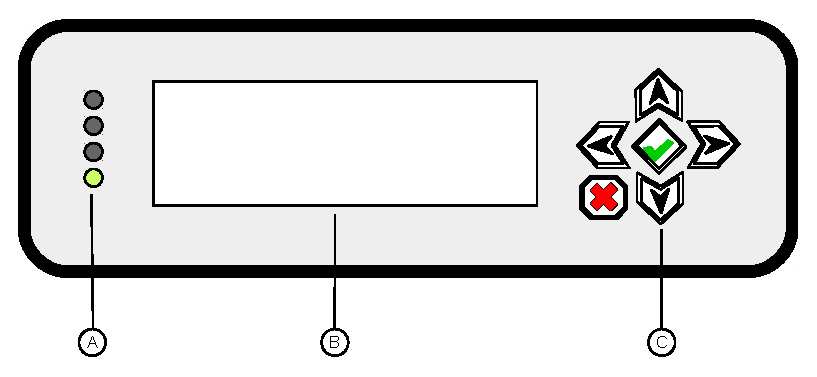
\psfig{file=figures/frontpanel.eps,silent=}
\caption{Front panel of the unit}
\end{figure}

\begin{itemize}
	\item[\mykey{A}] Status LEDs
	\item[\mykey{B}] LCD display
	\item[\mykey{C}] Keypad
\end{itemize}

The top line of the LCD display shows UTC date and time.
The date and time displayed will typically only be accurate to 1 s.
The contents of the second and third lines of the display depend on the display mode
\ref{ss:DisplayMode}.

The bottom line is reserved for notification of system alarms and either shows
`System OK' or `System Alarm'.
The LED beside this line will be red if there is a running alarm.
The other LEDs are currently unused.

\subsection{Using the front panel keypad \label{sKeypad} }

The keypad provides access to status information and limited control and configuration of the unit. 
It can be used to cleanly shut down or reboot the computer without logging in. 

System status is normally displayed on the screen.  
The menus are accessed by pressing any key. Menus are navigated  using the keypad:\\
%%\begin{table}[h]
\begin{tabular}{ll}
 \mykey{\begin{turn}{270}\ding{228}\end{turn}}& Move to next menu item \\
 \mykey{\begin{turn}{90}\ding{228}\end{turn}} & Move to previous menu item \\
 \mykey{\ding{228}}, \mykey{\ding{52}}& Select menu item \\
 \mykey{\begin{turn}{180}\ding{228}\end{turn}}  &Back to previous menu \\
 \mykey{\ding{54}}  & Back to the status display
\end{tabular}
%%\end{table}
\\
Escaping back to the status  after making a change will not undo the change.
Where a sub-menu lists a number of options, the currently selected option is flagged with an asterisk.

Dialogs are navigated using the cursor keys. A dialog will typically consist of a number of input fields. Some of these work like buttons and are selected using the \mykey{\ding{52}} key; others may require inputting a value and this is done by cycling through the possible values with the cursor keys. If you move out of an input field, focus will pass to the next valid input field. You can quit a dialog using the \mykey{\ding{54}} key. Any changes made in a dialog will not be applied if you quit it. If a menu or dialog has been inactive for more than 5 minutes, the display returns
to showing system status.

\subsection{Menus}

The menu hierarchy is shown below:

\begin{itemize}
	\item Setup
		\begin{itemize}
			\item LCD setup
				\begin{itemize}
					\item LCD settings
					\item LCD backlight time
				\end{itemize}
			\item Display mode
				\begin{itemize}
					\item GPS
					\item NTP
					\item GPSDO
				\end{itemize}
			\item Show IP addresses
		\end{itemize}
		
	\item Show alarms
	\item Show system info
	\item Restart
		\begin{itemize}
			\item GPS
			\item NTPD
			\item Reboot
			\item Power down
		\end{itemize}
\end{itemize}

\subsubsection{LCD setup}

The intensity and contrast of the LCD display can be set using this menu.
A timeout can also be set on the backlight.

\subsubsection{Display mode \label{ss:DisplayMode}}

The status information displayed by the unit in the second and third lines of the LCD display
can be selected as relating to either GPS, NTP or the GPSDO.

When in GPS mode, the identifiers of up
to 10 currently visible GPS space vehicles are displayed. 

When in NTP mode, the second line shows
the number of NTP packets received per minute. The third line shows information about
synchronization status, including leap second announcements.

In GPSDO mode, the second line shows whether the GPSDO is locked or not. 
The third line alternates between the `health' byte (\ref{sGPSDO}), and the estimated fractional frequency error 
(reported by the GPSDO) and the electronic frequency control (EFC) voltage, normalized to a maximum of 100.

\subsubsection{Show alarms}

This shows any currently running alarms as listed in \cc{/home/cvgps/logs/alarms}.

\subsubsection{Show system info}

This displays version and serial number information and the make of the installed oscillator.
This information is read from the file \cc{/usr/local/etc/sysinfo.conf} which has to be manually
updated as needed.
  
\subsubsection{Restart}

This allows the user to restart several processes (GPS common view logging and \cc{ntpd}) as well as reboot or power down the unit. 
You will be asked to confirm power down or reboot.

\pagebreak

\section{The rear panel}

\begin{figure}[h]
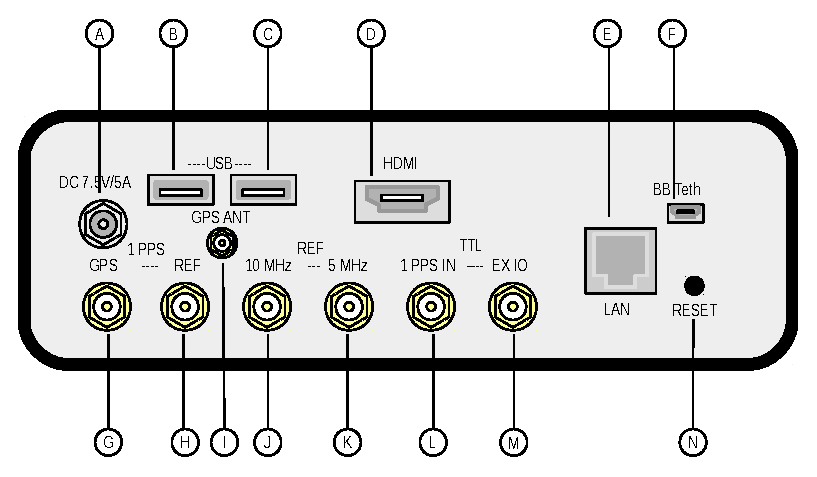
\psfig{file=figures/rearpanel.eps,silent=}
\caption{Rear panel of the unit}
\end{figure}

\begin{table}[h]
	\begin{tabular}{llll}
	& Function & Connector & Signal characteristics \\ 
	\mykey{A} & DC power input & & 7.5 V, 5A \\
	\mykey{B} & USB & & \\
	\mykey{C} & USB & & \\
	\mykey{D} & Video & HDMI & \\
	\mykey{E} & Network & RJ45 & \\
	\mykey{F} & BB USB network & & \\
	\mykey{G} & GPS 1 pps OUT & SMA & 5V DC supplied\\
	\mykey{H} & Reference 1 pps OUT & SMA & \\
	\mykey{I} & GPS antenna & SMB & \\
	\mykey{J} & Reference 10 MHz OUT& SMA & \\
	\mykey{K} & Reference 5 MHz OUT & SMA & \\
	\mykey{L} & 1 PPS IN & SMA & TTL\\
	\mykey{M} & General purpose I/O & SMA & TTL \\
	\mykey{N} & Beaglebone Black reset & &
	\end{tabular}
	\caption{Rear panel electrical connections}
\end{table}

If connected to a computer via the USB connector \mykey{F}, a network adapter should show up on your computer.
The \sysname{} will provide your computer with an IP address of either 192.168.7.1 or 192.168.6.1, depending on the type of USB network adapter
supported by your computer's operating system. The \sysname{} will reserve 192.168.7.2 or 192.168.6.2 for itself.

%% \enlargethispage*{48pt}
%% \pagebreak

\section{Installation}

\subsection{Operating environment}

The \sysname{} is designed for indoor use only and is neither water nor moisture-proof.
It should not be subjected to large mechanical shocks or excessive heat and dust.

\subsection{Install the GPS antenna and cable}

The unit supplies 5 V DC to the antenna. This can be changed to 3.3 V via a jumper J1.
More details are given in \ref{sAntenna}.

The GNSS antenna should be installed in a location with a clear
view of the sky above $10^{\circ}$. All exposed connections should be
weatherproofed. Make sure that all connections are tight but do not apply
excessive torque as this can result in connectors detaching from the cable.

A strain relief bulkhead is normally used for making the connection to the short 
`N'-terminated cable. 

\subsection{Make system connections}


\subsubsection{Network connection}

A network connection is not required for operation as a time-transfer system
but may be useful to the user for maintenance and downloading data files. Otherwise, 
a keyboard and monitor can be plugged in.

For operation as an NTP server, the unit will require a network connection.
The unit can operate using DHCP or with
a static IP address. The default is to use DHCP. The configured address can be conveniently found using the 
front panel menu.

A static IP can be set by using the system utility \cc{connmanctl} or by editing the file 
\cc{/etc/network/interfaces}.

\subsubsection{Keyboard and monitor}

A HDMI monitor and USB keyboard and mouse can be used with the \sysname{}. 
This will allow a console login \ref{sLoggingIn}.

The HDMI output may be disabled in some software images. If there is no HDMI output, TO DO. 

\subsubsection{Time and frequency signals}

Specifications of the various output signals are given in \ref{s:electricalspecs}.

\section{Logging in \label{sLoggingIn}}

The \sysname{} runs under Debian Linux. The desktop environment normally available has been disabled to reduce memory usage.
Familiarity with a command-line Linux environment is therefore essential for operating and maintaining
the \sysname{}. It is beyond the scope of this manual to provide a Linux tutorial. The reader should 
consult one of the many online resources that exist.

Login is via the user \cc{cvgps} (this name is used for historical reasons). 
The default password is supplied separately and you should change
this after logging in.

\section{The cvgps user}

The \cc{cvgps} user is the account used to log and process data.

It contains the 

Automatic operation is managed through the \cc{cvgps} \cc{crontab} file \ref{ss:crontab}.
\section{Checking  operation}

Upon startup, a number of alarms may be produced. 
All alarms should clear within five minutes of startup.
Information on alarms and troubleshooting hints are given in \ref{sAlarms}. Troubleshooting
will require logging into the system (\ref{sLoggingIn}).

You can check that logging of GNSS and counter data is occurring by looking in the directory 
\cc{/home/cvgps/raw}. Files in this directory are 

Processing of data takes place at UTC0015 daily. CGGTTS files will be placed in the 
\cc{/home/cvgps/raw} directory.

The \sysname{} is NTP-synchronized using the GPS receiver's time of day messages and its 1 pps. 
The \sysname{} operates on UTC. 
NTP operation can be checked using the command \cc{ntpq -p}. This should display 

\begin{table}[j]
\caption{Checking NTP operation}
\end{table}

\section{Essential configuration}

To produce CGGTTS files, the processing software needs accurate antenna coordinates.
These can be obtained from the \sysname{} receiver or by a separate survey.

\section{Updating the software}

Debian Linux is updated separately from the OpenTTP software.
Updating the kernel is a separate procedure. 

Updating the OpenTTP software is most conveniently done via the git repository.


\section{Securing the system}






%% ****************************************************************************************
\chapter{The reference platform hardware}
%% ****************************************************************************************

This chapter provides a more detailed description of the reference platform hardware.


\section{Antenna} \label{sAntenna}

The DC voltage supplied to the antenna is selectable as either 3.3 or 5 V with the jumper J1. 
The default is 5 V. Short circuit protection is 
provided via the $1 \Omega$ fusible resistor R25.

The NV08C-CSM has two antenna inputs ANT-A (active) and ANT-P (passive).
When the antenna is connected to ANT-P (default setting) the external DC power supply is used.
If the antenna is connected to ANT-A, the NV08-CSM board supplies 3.3 V DC and
short circuit protection is provided by the board.


\begin{figure}

	\centering
	
	\begin{subfigure}[t]{6cm}
		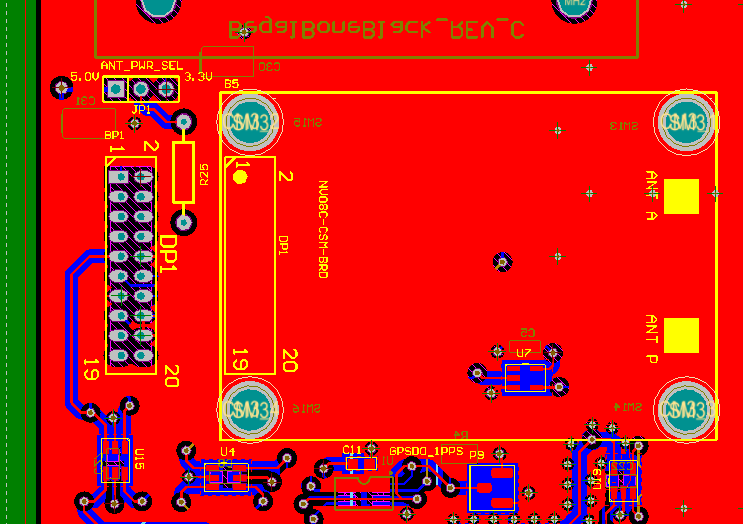
\includegraphics[width=6cm]{figures/antennavselpcb.png}
		\caption{Location of JP1 }
	\end{subfigure}
	
	\quad

	\begin{subfigure}[t]{6cm}
		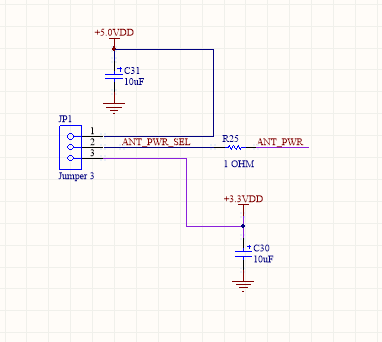
\includegraphics[width=6cm]{figures/antennavselcircuit.png}
		\caption{JP1 voltages}
	\end{subfigure}
	
	\caption{Selection of antenna voltage using JP1}
	
\end{figure}


\begin{figure}
\centerline{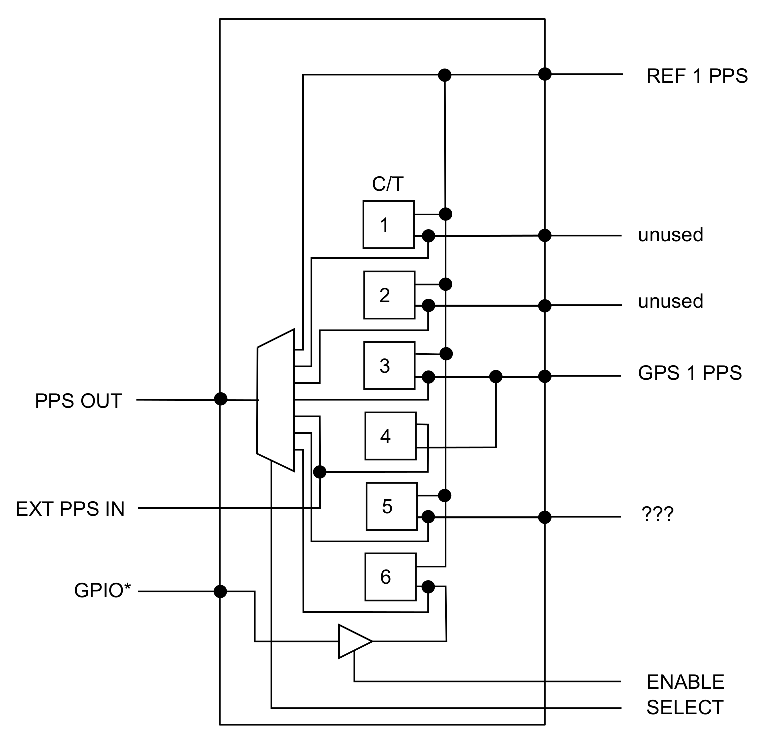
\includegraphics{figures/ottpcounter.eps}}
\end{figure}

\begin{table}
\begin{center}
\begin{tabular}{ll}
1 & channel 1 pps (unused)\\
2 & channel 2 pps (unused) \\
3 & channel 3 pps (GPS receiver)\\
4 & channel 4 pps (external pps)\\
5 & channel 5 pps (unused)\\
6 & channel 6 pps (GPIO)\\
7 & GPIO enabled\\
8 & Digital Clock Manager PLL is locked\\
\end{tabular}
\end{center}
\caption{Status LEDs}
\end{table}


%% ****************************************************************************************
\chapter{GPSCV software}
%% ****************************************************************************************


This chapter describes software related to GPSCV time-transfer.


\section{Software overview}

Time-transfer files are produced by \cc{mktimetx} from the GNSS receiver logs and counter/timer measurements.
The time-transfer files are in  RINEX observation  and CGGTTS format. 
Currently, CGGTTS-format files are only produced for GPS. 
Figure \ref{f:GPSCVProcessing} illustrates the processing chain TODO. 

The OpenTTP software suite is catalogued in Table \ref{t:OTTPSoftware}
\begin{table}
\begin{tabular}{l|l|l}
	& program & \\ 
	\hline
GPSCV processing  &  & \\
	& \hyperlink{h:mktimetx}{mktimetx} & core program\\
	& \hyperlink{h:runmktimetx}{runmktimetx.pl} & \\
	& \hyperlink{h:runr2cggttsv8}{runr2cggtsv8.py} & \\
	\hline
TIC logging & & \\
	& \hyperlink{h:hp5313xlog}{hp5313xlog.pl} &\\
	& \hyperlink{h:okxemlog}{okxemlog.pl} & \\
	& \hyperlink{h:prs10log}{prs10log.pl} & \\
	& \hyperlink{h:ticclog}{ticclog.py} & \\
	\hline
GNSS receiver logging & & \\
	&	\hyperlink{h:jnslog}{jnslog.pl} & Javad\\
	& \hyperlink{h:nvslog}{nv08log.pl} & NVS\\
	& \hyperlink{h:restlog}{restlog.pl} & Trimble Resolution T\\
	& \hyperlink{h:ublox9log}{ublox9log.py} & ublox\\
	& \hyperlink{h:ubloxlog}{ubloxlog.pl} & ublox\\
GNSS receiver utilities & & \\
	& \hyperlink{h:jnsextract}{jnsextract.pl} & \\
	& \hyperlink{h:nv08extract}{nv08extract.pl} & \\
	& \hyperlink{h:nv08info}{nv08info.pl} & \\
	& \hyperlink{h:restextract}{restextract.pl} & \\
	& \hyperlink{h:restinfo}{restinfo.pl} & \\
	& \hyperlink{h:ubloxextract}{ubloxextract.py} & \\
	& \hyperlink{h:ubloxmkdev}{ubloxmkdev.py} & \\
	\hline
Analysis tools & & \\
	& \hyperlink{h:cggttsqc}{cggttsqc.py} & \\
	& \hyperlink{h:cmpcggtts}{cmpcggtts.py} & \\
	& \hyperlink{h:editcggtts}{editcggtts.py} & \\
	& \hyperlink{h:editrnxnav}{editrnxnav.py} & \\
	& \hyperlink{h:editrnxobs}{editrnxobs.py} & \\
	& \hyperlink{h:ticqc}{ticqc.py} & \\
Miscellaneous & & \\
  & \hyperlink{h:log1Wtemp}{log1Wtemp.pl} & \\ 
	\hline
\end{tabular}
\caption{GPSCV software overview \label{t:OTTPSoftware} }
\end{table}

\section{crontab \label{ss:crontab}}

Automatic logging, processing and archival of data is co-ordinated via the user \cc{cvgps}' \cc{crontab}.

A minimal \cc{crontab} for the user \cc{cvgps} looks like this:
\begin{lstlisting}
# Check that all logging is running every 5 minutes
*/5 * * * * /usr/local/bin/kickstart.pl # See ~/etc/kickstart.conf

# Run the processing of the data at 00:15
15 0 * * * nice $HOME/bin/runmktimetx.pl >/dev/null 2>&1 

# Give the processing some time to complete, then zip the files at 00:45
45 0 * * * nice $HOME/bin/gziplogs.pl >/dev/null 2>&1

# Check the status of the system once a day, just before the day rollover
56 23 * * * $HOME/bin/checkstatus.pl >$HOME/lockStatusCheck/status.dat
\end{lstlisting}
showing the three essential processes of logging, processing and archival of data.

The active crontab can be examined with the command \cc{crontab -l}. 
A default \cc{crontab} is saved in \cc{/home/cvgps/etc/crontab}. 

\section{Configuration file format \label{sConfigFileFormat}}

Configuration files use a common format and are plain text files, designed to be easily edited via a command-line
editor because in many applications, only shell access to the system will be available.

The file is usually divided into sections, with section names delimited by square brackets [ ]. Entries in each section
are of the form:
\begin{lstlisting}
key = value
\end{lstlisting}
For example,
\begin{lstlisting}
[Receiver]
manufacturer = Trimble
model = Resolution T
\end{lstlisting}
defines a section \cc{Receiver} and the two keys: \cc{manufacturer} and \cc{model}. 

The notation \cc{Section::Key} is used to fully specify keys. For example,
\cc{Receiver::model} and \cc{Receiver::manufacturer} specify the two keys above.

Keys and section names are not case-sensitive. In particular, the python and Perl libraries
which provide functions for reading the configuration files convert keys and section names to lower case.
The case of key values is preserved, since this may be signficant eg path names.

Leading and trailing whitespace is removed from keys, key values and section names.

Comments begin with a `\#'. 

Some keys define a list of sections. 
For example, the comma-separated list of values for \cc{CGGTTS::outputs} 
\begin{lstlisting}
[CGGTTS]
outputs = c1-code,p1-code,p2-code
\end{lstlisting}
defines three sections: \cc{c1-code}, \cc{p1-code}, and \cc{p2-code}.
This is a bodge which would be more elegantly addressed using an extensible format like XML, 
but it has proven to be sufficient for our needs.

\subsection{Paths} \label{s:ConfigFilePaths}

Paths to files  specified in a configuration file are constructed with the following 
precedence:
\begin{enumerate}
\item If the path begins with a leading slash, then it is interpreted as an absolute path
\item If a non-absolute path is specified, it is interpreted as being relative to 
	the users's home directory (or where the configuration file allows specification of a different root path eg in \hyperlink{h:rootpath}{gpscv.conf}, relative to that root path) 
\item Otherwise, the default path is used.
\end{enumerate}
Most software in OpenTTP follows these conventions.

\section{Data file formats \label{s:DataFileFormat}}

\subsection{GPS receiver}

This text file records messages from the GPS receiver. 
The native format of the messages can be a mix of ASCII and binary messages.
Binary messages are hexadecimal-encoded for saving in the log file. 
Some logging scripts record ancillary information, such as commands sent to the receiver. 
Comments in the log file are allowed, prefaced by a `\#' character. 
The `@' character is used to tag lines containing special information that needs to be parsed by
the processing software.

Messages are successive lines of the form:
\begin{lstlisting}
<message_id> <time_stamp> <message>
\end{lstlisting}
\textit{Example:}
\begin{lstlisting}
TO 00:00:02 cdfbc75a9a8c353fc5
\end{lstlisting}

Hex encoding of binary messages results in much larger files but these compress to a size not much larger
than the original binary data.

\subsection{Time-interval counter \label{s:TICformat}}

This text file records the difference between GNSS receiver and the Reference Oscillator 1 pps,
measured each second. Entries are successive lines of the form:
\begin{lstlisting}
<time_of_day> <time_difference>
\end{lstlisting}
where the time difference is in seconds.\\
\textit{Example:}
\begin{lstlisting}
00:00:04  +4.0821E-006 
\end{lstlisting}

\section{gpscv.conf - the core configuration file \label{sgpscvconf} }

A single configuration file, \cc{gpscv.conf}, provides configuration information to most of the
OpenTTP software. 
\cc{gpscv.conf} is used by \cc{mktimetx}, receiver logging scripts, TIC logging scripts,receiver utilities and so on.

It uses the format described in \ref{sConfigFileFormat}.

\begin{table}[ht]
\begin{tabular}{l|p{10cm}}
Section & Key \\ \hline
\hyperlink{h:antenna}{Antenna} & antenna number, antenna type, 
				delta H, delta N, delta E, frame,
				marker name, marker number,
				X, Y, Z\\ \hline
\hyperlink{h:cggtts}{CGGTTS} & BIPM cal id, comments, create, 
         ephemeris, ephemeris file, ephemeris path,
         internal delay, lab id, maximum DSG, minimum elevation,
         minimum track length, naming convention, outputs, reference,
         receiver id, revision date, version,
         code, constellation, path
         \\ \hline
\hyperlink{h:delays}{Delays}  & antenna cable, reference cable 
         \\ \hline
\hyperlink{h:counter}{Counter} & file extension, GPIB address, header generator, lock file,
         logger, logger options, okxem channel, port
				\\ \hline
\hyperlink{h:misc}{Misc}    & gzip
				\\ \hline
\hyperlink{h:paths}{Paths} & CGGTTS, counter data, processing log, receiver data, RINEX, tmp
				\\ \hline
\hyperlink{h:receiver}{Receiver} & configuration, elevation mask, logger, logger options, 
				 manufacturer, model, observations, 
         port, pps offset, synchronization, pps synchronization delay,
         status file, timeout, version
				\\ \hline
\hyperlink{h:reference}{Reference} & file extension, logging interval, log path, log status, oscillator, power flag, status file
        \\ \hline
\hyperlink{h:rinex}{RINEX}  & agency, create, observer, version
				\\ \hline
\end{tabular}
\caption{Summary of \cc{gpscv.conf} entries}
\end{table}

\subsection{[Antenna] section}

Entries used to create the RINEX header are:
\begin{itemize}
\item antenna number
\item antenna type
\item delta H, delta E, delta N
\item marker name
\item marker number
\item X,Y,Z
\end{itemize}

Entries used to create the CGGTTS header are:
\begin{itemize}
\item X,Y,Z
\end{itemize}

\hypertarget{h:antenna}{}
{\bfseries antenna number}\\
This appears as ANTNUM in the RINEX header.\\
\textit{Example:}
\begin{lstlisting}
antenna number = A567456
\end{lstlisting}

{\bfseries antenna type}\\
This appears as ANTTYPE in the RINEX header.\\
\textit{Example:}
\begin{lstlisting}
antenna type = Ashtec
\end{lstlisting}

{\bfseries delta H}\\
This appears as DELTA H in the RINEX header.\\
\textit{Example:}
\begin{lstlisting}
delta H = 0.0
\end{lstlisting}

{\bfseries delta E}\\
This appears as DELTA E in the RINEX header.\\
\textit{Example:}
\begin{lstlisting}
delta E = 0.0
\end{lstlisting}

{\bfseries delta N}\\
This appears as DELTA N in the RINEX header.\\
\textit{Example:}
\begin{lstlisting}
delta N = 0.0
\end{lstlisting}

{\bfseries frame}\\
This appears as FRAME in the CGGTTS header.\\
\textit{Example:}
\begin{lstlisting}
frame = ITRF2010
\end{lstlisting}

{\bfseries marker name}\\
This appears as MARKER NAME in the RINEX header.\\
\textit{Example:}
\begin{lstlisting}
marker name =
\end{lstlisting}

{\bfseries marker number}\\
This appears as MARKER NUMBER in the RINEX header.\\
\textit{Example:}
\begin{lstlisting}
marker number =
\end{lstlisting}

{\bfseries X}\\
This appears as X in the CGGTTS header and APPROX POSITION XYZ in the RINEXheader.\\
\textit{Example:}
\begin{lstlisting}
X = +4567890.123
\end{lstlisting}

{\bfseries Y}\\
This appears as Y in the CGGTTS header and APPROX POSITION XYZ in the RINEXheader.\\
\textit{Example:}
\begin{lstlisting}
Y = +2345678.90
\end{lstlisting}

{\bfseries Z}\\
This appears as Z in the CGGTTS header and APPROX POSITION XYZ in the RINEXheader.\\
\textit{Example:}
\begin{lstlisting}
Z = -1234567.890 
\end{lstlisting}


\subsection{[CGGTTS] section }

\hypertarget{h:cggtts}{Entries} in this section control the format and content of CGGTTS files 
and filtering applied to CGGTTS tracks in the final output.

To create CGGTTS output you must enable it: 


{\bfseries outputs}\\
This defines a list of sections which in turn define the desired CGGTTS outputs.\\
\textit{Example:}
\begin{lstlisting}
outputs = CGGTTS-GPS-C1,CGGTTS-GPS-P1,CGGTTS-GPS-P2
\end{lstlisting}

A CGGTTS v2E header looks like:
\begin{lstlisting}
CGGTTS     GENERIC DATA FORMAT VERSION = 2E
REV DATE = 2018-03-20
RCVR = NVS NV08 undefined 1999 mktimetx,v0.1.4
CH = 32
IMS = 99999
LAB = NMIA
X = -4648239.852 m
Y = +2560635.623 m
Z = -3526317.023 m
FRAME = ITRF2008
COMMENTS = none
INT DLY = 0.0 ns (GPS C1)     CAL_ID = none
CAB DLY = 0.0 ns
REF DLY = 0.0 ns
REF = UTC(AUS)
CKSUM = 1A
\end{lstlisting}

Entries in the header than can be defined in the CGGTTS section are as below. 

{\bfseries comments}\\
This defines a single COMMENTS line in the CGGTTS header.
The output line will be truncated at 128 characters.\\
\textit{Example:}
\begin{lstlisting}
comments = none
\end{lstlisting}

{\bfseries lab }\\
This defines the LAB line.\\
\textit{Example:}
\begin{lstlisting}
lab = NMI
\end{lstlisting}

{\bfseries reference}\\
This defines REF in the CGGTTS header.\\
\textit{Example:}
\begin{lstlisting}
reference = UTC(XXX)
\end{lstlisting}

{\bfseries revision date}\\
This defines REV DATE in the CGGTTS header. It must be in the format YYYY-MM-DD.\\
\textit{Example:}
\begin{lstlisting}
revision date = 2015-12-31
\end{lstlisting}


{\bfseries create}\\
This defines whether or not CGGTTS files will be generated by \cc{mktimetx}.\\
\textit{Example:}
\begin{lstlisting}
create = yes
\end{lstlisting}

{\bfseries ephemeris}\\
This defines whether to use the receiver-provided ephemeris or a user-provided ephemeris (via a RINEX navigation file).
If a user-provided ephemeris is specified then \cc{ephemeris path} and \cc{ephemeris file} 
must also be specified.\\
\textit{Example:}
\begin{lstlisting}
ephemeris = receiver
\end{lstlisting}

{\bfseries ephemeris file}\\
This specifies a pattern for user-provided RINEX navigation files.
Currently, only patterns of the form \cc{XXXXddd0.yyn} are recognized.\\
\textit{Example:}
\begin{lstlisting}
ephemeris file = brdcddd0.yyn
\end{lstlisting}

{\bfseries ephemeris path}\\
This specifies the path to user-provided RINEX navigation files.\\
\textit{Example:}
\begin{lstlisting}
ephemeris path = igsproducts
\end{lstlisting}

{\bfseries lab id}\\
This defines the two-character lab code used for creating BIPM-style file names, as per the V2E specification.\\
\textit{Example:}
\begin{lstlisting}
lab id = AU
\end{lstlisting}

{\bfseries maximum DSG}\\
CGGTTS tracks with DSG lower than this will be filtered out. 
The units are ns.\\
\textit{Example:}
\begin{lstlisting}
maximum DSG = 10.0
\end{lstlisting}

{\bfseries minimum elevation}\\
CGGTTS tracks with elevations lower than this will be filtered out. 
The units are degrees.\\
\textit{Example:}
\begin{lstlisting}
minimum elevation = 10
\end{lstlisting}

{\bfseries minimum track length}\\
CGGTTS tracks shorter than this will be filtered out. Tracks meeting the criterion are not necessarily contiguous.
The units are seconds.\\
\textit{Example:}
\begin{lstlisting}
minimum track length = 390
\end{lstlisting}

{\bfseries maximum URA}\\
GPS ephemerides with URA greater than this will not be used. 
They will still be written to RINEX navigation files, however.\\
\textit{Example:}
\begin{lstlisting}
maximum URA = 3.0
\end{lstlisting}

{\bfseries naming convention}\\
Defines the CGGTTS file naming convention. Valid options are `plain' (MJD.cctf) and `BIPM' styles.
The \cc{lab id} and \cc{receiver id} should be defined in conjunction with BIPM-style filenames.\\
\textit{Example:}
\begin{lstlisting}
naming convention = BIPM
\end{lstlisting}

{\bfseries receiver id}\\
This defines the two-character receiver code used for creating BIPM-style file names, 
as per the V2E specification.\\
\textit{Example:}
\begin{lstlisting}
receiver is = 01
\end{lstlisting}

{\bfseries version}\\
This defines the version of CGGTTS output. Valid versions are v1 and v2E. 
The \cc{lab id} and \cc{receiver id} should be defined in conjunction with v2E ouput\\
\textit{Example:}
\begin{lstlisting}
version = v2E
\end{lstlisting}


\subsubsection{CGGTTS output sections}

Multiple CGGTTS outputs can be defined, allowing for different constellation and signal combinations.
An example of a CGGTTS output section is as follows:
\begin{lstlisting}
[CGGTTS-GPS-C1]
constellation=GPS
code=C1
path=cggtts
BIPM cal id = none
internal delay = 11.0
\end{lstlisting}

{\bfseries BIPM cal id}\\
This defines CAL\_ID for the internal delay, as used in v2E CGGTTS headers.\\
\textit{Example:}
\begin{lstlisting}
BIPM cal id = none
\end{lstlisting}

{\bfseries code}\\

CGGTTS codes can be specified using either the two letter code, for example `C1' as described in the CGGTTS V2E 
specification, or three letter RINEX v3.03 observation codes.
\begin{table}
\begin{tabular}{ll}
	CGGTTS name	 & RINEX name \\ \hline
	C1 & C1C \\
	P1 & C1P \\
	E1 & C1C \\
	B1 & C2I \\
	C2 & C2C \\
	P2 & C2P \\
	B2 & C7I 
\end{tabular}
\caption{Correspondence of CGGTTS and RINEX signal names.}
\end{table}
\textit{Example:}
\begin{lstlisting}
code = P1+P3
\end{lstlisting}

{\bfseries constellation}\\
This defines the GNSS constellation. Only GPS is supported currently for CGGTTS generation.\\
\textit{Example:}
\begin{lstlisting}
constellation = GPS
\end{lstlisting}

{\bfseries internal delay}\\
This defines INT DLY in the CGGTTS header. The units are ns.\\
\textit{Example:}
\begin{lstlisting}
INT DLY = 0.0
\end{lstlisting}

{\bfseries path}\\
This defines the directory in which output files are placed.\\
\textit{Example:}
\begin{lstlisting}
path = cggtts
\end{lstlisting}

In v1 CGGTTS files, the delays are specified via INT DLY, CAB DLY and ANT DLY.  
For v2E files, the delays may be specified via the `system delay' and `total delay'.
If multiple delays (eg both internal and system delay are present) are defined in
\cc{gpscv.conf}, the precedence order is internal, system and then total delay.

The entries used to specify system and total delay are:\\

{\bfseries system delay}\\
This defines SYS DLY in the CGGTTS header. The units are ns.\\
\textit{Example:}
\begin{lstlisting}
SYS DLY = 0.0
\end{lstlisting}

{\bfseries total delay}\\
This defines TOT DLY in the CGGTTS header. The units are ns.\\
\textit{Example:}
\begin{lstlisting}
TOT DLY = 0.0
\end{lstlisting}

\subsection{[Counter] section}

\hypertarget{h:counter}{}

{\bfseries file extension}\\
This defines the extension used for time interval measurement files.
The default is `tic'.\\
\textit{Example:}
\begin{lstlisting}
file extension = tic
\end{lstlisting}

{\bfseries configuration}\\ \hypertarget{h:counter_configuration}{}
This sets a configuration file for the counter. Its contents are defined by the calling script.
In the case of HP5313x counters for example,
it lists SCPI commands sent to initiliaze the counter.\\
\textit{Example:}
\begin{lstlisting}
configuration = etc/hp53131.conf
\end{lstlisting}

{\bfseries flip sign}\\
The processing software eg \cc{mktimetx} assumes that TIC measurements are started by the reference
and stopped by the GNSS receiver. If you need to invert the sign of the measurements, set the option
`flip sign' to `yes',
\textit{Example:}
\begin{lstlisting}
flip sign = no 
\end{lstlisting}

{\bfseries GPIB address}\\ \hypertarget{h:counter_gpib_address}{}
For GPIB devices, the GPIB address must be defined.\\
\textit{Example:}
\begin{lstlisting}
GPIB address = 3
\end{lstlisting}

{\bfseries GPIB converter}\\  \hypertarget{h:counter_gpib_converter}{}
This defines the GPIB interface converter (eg RS232 to GPIB).
Currently the only valid values is `Micro488'.\\
\textit{Example:}
\begin{lstlisting}
GPIB converter = Micro488
\end{lstlisting}

{\bfseries header generator}\\
A header for the log file can be optionally added to the log file, using the output
of a user provided script. Output should be to \cc{stdout}.
Each line will have a ``\#'' automatically prepended to it.\\
\textit{Example:}
\begin{lstlisting}
header generator = bin/myticheader.pl
\end{lstlisting}

{\bfseries lock file}\\
This defines the device lock file, used to prevent multiple instances of the logger
from being started.\\
\textit{Example:}
\begin{lstlisting}
lockfile = okxem.gpscv.lock
\end{lstlisting}

{\bfseries logger}\\
This defines the counter logging script.\\
\textit{Example:}
\begin{lstlisting}
logger = okxemlog.pl
\end{lstlisting}

{\bfseries logger options}\\
This defines options passed to the counter logging script.\\
\textit{Example:}
\begin{lstlisting}
logger options =
\end{lstlisting}

{\bfseries mode}\\ \hypertarget{h:counter_mode}{}
This defines the operating mode of the counter.
Valid values are \cc{timestamp} and \cc{time interval}
Currently, this is only used by the TAPR TICC.\\
\textit{Example:}
\begin{lstlisting}
mode = timestamp
\end{lstlisting}

{\bfseries okxem channel}\\ \hypertarget{h:counter_okxem_channel}{}
The OpenTTP counter is multi-channel so the channel to use (1-6) must be specified.\\
\textit{Example:}
\begin{lstlisting}
okxem channel=3
\end{lstlisting}

{\bfseries port}\\ \hypertarget{h:counter_port}{}
This defines the port used to communicate with the counter. It's value depends on the type of counter. 
For the XEM6001, it's a Unix socket. For serial devices, it's a device name like
\cc{/dev/ttyUSB0}.\\
\textit{Example:}
\begin{lstlisting}
# this is the port used by okcounterd
port = 21577 
\end{lstlisting}

{\bfseries timestamp format}\\ \hypertarget{h:counter_timestamp_format}{}
This controls the format of timestamps used in the counter log file.
Valid values are \cc{unix} and \cc{time of day}.
Currently, this is only used by the TAPR TICC.\\
\textit{Example:}
\begin{lstlisting}
timestamp format = time of day
\end{lstlisting}

\subsection{[Misc] section}

\hypertarget{h:misc}{}

{\bfseries gzip}\\
Defines the compression/decompression program used in conjunction with counter and receiver log files.\\
\textit{Example:}
\begin{lstlisting}
gzip = /bin/gzip 
\end{lstlisting}

\subsection{[Delays] section}

\hypertarget{h:delays}{}

{\bfseries antenna cable}\\
This is ANT DLY as used in the CGGTTS header. Units are ns.\\
\textit{Example:}
\begin{lstlisting}
antenna cable = 0.0
\end{lstlisting}

{\bfseries reference cable}\\
This is REF DLY as used in the CGGTTS header. Units are ns.\\
\textit{Example:}
\begin{lstlisting}
reference cable = 0.0
\end{lstlisting}

\subsection{[Paths] section} 

\hypertarget{h:paths}{}

Paths follow the rules described in .

{\bfseries root}\\ \hypertarget{h:rootpath}{}
Defines the root path to be used with all other paths, unless they are specified as absolute paths.
As with other paths specified in \cc{gpscv.conf}, it is interpreted as being relative to the user's
home directory, unless prefaced with a `/'.\\
\textit{Example:}
\begin{lstlisting}
root = test/newreceiver
\end{lstlisting}

{\bfseries CGGTTS}\\
Defines the default directory used for CGGTTS files.
This is typically overridden by the output directory that can be  defined in each CGGGTS output section.\\
\textit{Example:}
\begin{lstlisting}
CGGTTS = cggtts
\end{lstlisting}

{\bfseries counter data}\\
Defines the directory used for TIC data files.\\
\textit{Example:}
\begin{lstlisting}
counter data = raw
\end{lstlisting}

{\bfseries processing log}\\
Defines the directory where the \cc{mktimetx} processing log is written.\\
\textit{Example:}
\begin{lstlisting}
processing log = logs
\end{lstlisting}

{\bfseries receiver data}\\
Defines the directory used for GNSS receiver raw data files.\\
\textit{Example:}
\begin{lstlisting}
receiver data = raw
\end{lstlisting}

{\bfseries RINEX}\\
Defines the directory used for RINEX files.\\
\textit{Example:}
\begin{lstlisting}
RINEX = rinex
\end{lstlisting}

{\bfseries tmp}\\
Defines the directory used for intermediate and debugging files.\\
\textit{Example:}
\begin{lstlisting}
tmp = tmp
\end{lstlisting}

{\bfseries onewire temp data}\\
Defines the directory used to write temperature logs.\\
\textit{Example:}
\begin{lstlisting}
onewiretemp data = raw/onewire
\end{lstlisting}

{\bfseries uucp lock}\\
Sets the directory used to write UUCP lock files. UUCP lock files are used with serial devices to prevent
other processes (eg \cc{minicom}) opening the serial port while it is in use. The default is \cc{/var/lock}
but this varies with the operating system and its version so you will need to check this.\\
\textit{Example:}
\begin{lstlisting}
# This is for Debian
uucp lock = /var/run/lock
\end{lstlisting}

{\bfseries rinex l1l2}\\ \hypertarget{h:rinex_l1l2}{}
Defines the directory used to write RINEX files with all observations, typically so that precise antenna coordinates
can be obtained. This is only used with dual frequency Javad receivers.\\
\textit{Example:}
\begin{lstlisting}
rinex l1l2 = rinex/l1l2
\end{lstlisting}


\subsection{[Receiver] section \label{sgcreceiver}}

\hypertarget{h:receiver}{}

{\bfseries configuration}\\
\\
\textit{Example:}
\begin{lstlisting}
configuration = etc/rx.conf
\end{lstlisting}

{\bfseries elevation mask}\\
This sets an elevation mask for tracking os satellites - below this elevation, satellites
are ignored. The units are degrees. This may not be implemented for all receivers.\\
\textit{Example:}
\begin{lstlisting}
elevation mask = 0
\end{lstlisting}

{\bfseries logger}\\
This is the script used to configure and log messages from the GNSS receiver.\\
\textit{Example:}
\begin{lstlisting}
logger = jnslog.pl
\end{lstlisting}

{\bfseries logger options}\\
These are options passed to the receiver logging script.\\
\textit{Example:}
\begin{lstlisting}
logger options =
\end{lstlisting}

{\bfseries manufacturer}\\
This defines the manufacturer of the receiver. Together with the model and version, 
this sets how data from the receiver is processed. For a list of supported receivers
see XX.\\
\textit{Example:}
\begin{lstlisting}
manufacturer = Javad
\end{lstlisting}

{\bfseries model}\\
This is the receiver model.For a list of supported receivers
see XX.\\
\textit{Example:}
\begin{lstlisting}
model = HE_GGD
\end{lstlisting}

{\bfseries version}\\
This can be used to identify the firmware version in use, for example.\\
\textit{Example:}
\begin{lstlisting}
version = 2.6.1
\end{lstlisting}

{\bfseries observations}\\
This is a list of GNSS systems which will be tracked by the receiver. 
In some applications where a multi-GNSS receiver is used, it may be desirable to track
only one GNSS system so this sets which system is used.
More generally, low-end multi-GNSS receivers are typically only capable of tracking
certain combinations of GNSS systems so this is used to select the required combination.
\textit{Example:}
\begin{lstlisting}
observations = GPS
\end{lstlisting}

{\bfseries port}\\
This is the serial port used for communication with the receiver.\\
\textit{Example:}
\begin{lstlisting}
port = /dev/ttyS0
\end{lstlisting}

{\bfseries pps offset}\\ 
This is an offset programmed into the GNSS receiver. Its purpose is to ensure that the counter
triggers correctly, particularly HP5313x counters, which will only trigger every two seconds if the 
start trigger slips slightly behind the stop trigger. Suitable values are determined by the long-term stability of the
reference, compared with GPS.
The units are ns.\\
\textit{Example:}
\begin{lstlisting}
pps offset = 3500
\end{lstlisting}

{\bfseries configuration}\\ \hypertarget{h:configuration}{}
This specfies a file to be used to configure the receiver. Currently, it is only used
with Javad receivers.\\
\textit{Example:}
\begin{lstlisting}
configuration = rx.cfg
\end{lstlisting}

{\bfseries pps synchronization}\\ \hypertarget{h:pps_synchronization}{}
This is a Javad-specific option. The logging script will force a synchronization of the receiver's
internal time scale with the input 1 pps.\\
\textit{Example:}
\begin{lstlisting}
pps synchronization = no
\end{lstlisting}

{\bfseries pps synchronization delay}\\ \hypertarget{h:pps_synchronization_delay}{}
This is a Javad-specific option. Synchronization of the receiver's
internal time scale with the input 1 pps is delayed for this time after reset of the receiver.
The units are seconds.\\
\textit{Example:}
\begin{lstlisting}
pps synchronization delay = 300
\end{lstlisting}

{\bfseries status file}\\
The status file contains a summary of the current state of the receiver,tyically at least the
currently visible GNSS satellites. Other software, for example \cc{lcdmonitor}, uses this information.\\
\textit{Example:}
\begin{lstlisting}
status file = logs/rx.status
\end{lstlisting}

{\bfseries timeout}\\
The logging script will time out and exit if no messages are received for this period.\\
\textit{Example:}
\begin{lstlisting}
timeout = 60
\end{lstlisting}

{\bfseries sawtooth phase}\\
This defines which pps the sawtooth correction is to be applied to.
Valid values are `current second', `next second' and `receiver specified'.
`Current' means for the pps just generated.\\
\textit{Example:}
\begin{lstlisting}
sawtooth phase = current second
\end{lstlisting}

{\bfseries year commissioned}\\
The year the receiver was commissioned. This is used in the CGGTTS header.\\
\textit{Example:}
\begin{lstlisting}
year commissioned = 1999
\end{lstlisting}

\subsection{[Reference] section}

\hypertarget{h:reference}{}

{\bfseries file extension}\\ \hypertarget{h:reference_file_extension}{}
This defines the extension used for Reference status logs.\\
\textit{Example:}
\begin{lstlisting}
file extension = .rb
\end{lstlisting}

{\bfseries logging interval}\\ \hypertarget{h:reference_logging_interval}{}
This defines the interval between status file updates. The units are seconds.\\
\textit{Example:}
\begin{lstlisting}
logging interval = 60
\end{lstlisting}

{\bfseries log path}\\ \hypertarget{h:reference_log_path}{}
This defines where status logs are written to.\\
\textit{Example:}
\begin{lstlisting}
log path = raw
\end{lstlisting}

{\bfseries log status}\\ \hypertarget{h:reference_log_status}{}
This enables status logging of the Reference.\\
\textit{Example:}
\begin{lstlisting}
log status = yes
\end{lstlisting}

{\bfseries oscillator}\\
This identifies the installed oscillator, so that device-specific handling can be implemented.\\
\textit{Example:}
\begin{lstlisting}
oscillator = PRS10
\end{lstlisting}

{\bfseries power flag}\\ \hypertarget{h:reference_power_flag}{}
This defines the file used to flag that the Reference has lost power, and needs rephasing.
Currently, this only has meaning for the PRS10. It is used ntpd to disable the refclock
corresponding to the PRs10's 1 pps.\\
\textit{Example:}
\begin{lstlisting}
power flag = logs/prs10.pwr
\end{lstlisting}

{\bfseries status file}\\ \hypertarget{h:reference_status_file}{}
In the case of the PRS10, this consists of the six status bytes and sixteen ADC values.\\
\textit{Example:}
\begin{lstlisting}
status file = logs/prs10.status
\end{lstlisting}


\subsection{[RINEX] section}

\hypertarget{h:rinex}{Entries} in this section control the format and content of RINEX files.
RINEX observation and navigation files in version 2 and version 3 formats can be produced.
RINEX observations 

{\bfseries agency}\\
This specifies the value of the AGENCY field which appears in RINEX observation file headers.\\
\textit{Example:}
\begin{lstlisting}
agency = MY AGENCY
\end{lstlisting}

{\bfseries create}\\
This defines whether or not RINEX files will be generated.\\
\textit{Example:}
\begin{lstlisting}
create = yes
\end{lstlisting}

{\bfseries force v2 name}\\
This forces a V2 name for V3 RINEX output.\\
\textit{Example:}
\begin{lstlisting}
force v2 name = no
\end{lstlisting}

{\bfseries observer}\\
Normally, only code observations are output by mktimetx. 
To output phase observations, set this to 'all'.\\
\textit{Example:}
\begin{lstlisting}
observations = code
\end{lstlisting}

{\bfseries observer}\\
This specifies the value of the OBSERVER field which appears in RINEX observation file headers.
If the observer is specified as `user' then the environment variable USER is used.\\
\textit{Example:}
\begin{lstlisting}
observer = user
\end{lstlisting}

{\bfseries version}\\
This  specifies the version of the RINEX output. Valid versions are 2 and 3.\\
\textit{Example:}
\begin{lstlisting}
version = 2
\end{lstlisting}





General notes

NVS

Note that this receiver uses UTC as the reference timescale to report time stamps.

This receiver reports a measurement time for observation a few hundred ms prior to the upcoming
second.

Trimble

 

Internals

One aspect to keep straight is that three timescales are used in the software:
PC time
UTC
GPS time

PC time is used only to match TIC and GNSS observations. Time stamps recorded in measurement files do
not have a fractional seconds part. The latency of the various signals (eg GPS messages 
for a second are always output after the beginning of the second) and their logging by the host PC 
means that this is no ambiguity during normal operation.

UTC time is used for CGGTTS generation.

GPS time is used for various calculations and for RINEX observations.

/subsection{Application.cpp}

Matched measurements are stored in a vector whose index corresponds to UTC time-of-day.

/subsection{CGGTTS.cpp}



/section{Adding support for a new receiver}

Conventions

A counter/timer measurement must be started by REF and stopped by GPS.
There is an option in gpscv.conf to reverse the sign of this.

The sawtooth correction is ADDED to the counter/timer measurement.


Debugging and validation

It can be useful to look at how well the receiver recovers GPS time - this is easily done by
using the option --disable-tic. The sawtooth-corrected TIC measurement is then set to zero.

REFSYS values noisy at the hundreds of ns level may indicate an off by one error in assigned time stamps.


\section{runmktimetx.pl \label{runmktimetx}}

\hypertarget{h:runmktimetx}{}

\cc{runmktimetx.pl} provides a convenient way to process multiple days of data and to run any missed processing.

\cc{runmktimetx.pl} uses \cc{gpscv.conf}. There are no entries in \cc{gpscv.conf} specific to \cc{runmktimetx.pl}

\cc{runmktimetx.pl} doesn't produce a log file.
	
\subsection{usage}
\cc{runmktimetx.pl} is normally run as a \cc{cron} job.

To run \cc{runmktimetx.pl} on the command line, use
\begin{lstlisting}[mathescape=true]
runmktimetx.pl [option] $\ldots$ [Start MJD  [Stop MJD]]
\end{lstlisting}

\cc{Start MJD} and \cc{Stop MJD} specify the range of MJDs to process.
If a single MJD is specified, then data for that day is processed. If no
MJD is specified, the previous day's data is processed.

The options are:
\begin{description*}
	\item[-a \textless{file}\textgreater]  extend check for missed processing back \cc{n} days 
		(the default is~7)
	\item[-c \textless{file}\textgreater] use the specified configuration file
	\item[-d]	run in debugging mode
	\item[-h]	print help and exit
	\item[-x] run missed processing
	\item[-v]	print version information and exit
\end{description*}



\section{runr2cggttsv8.py}

\hypertarget{h:runr2cggttsv8}{}

\cc{runr2cggttsv8.py}  can be used to automate the running of
\cc{r2cggtts} a program commonly used for generating CGGTTS files from RINEX files.
In particular, given an MJD, it will copy and rename RINEX observation and navigation files
to the files needed by \cc{r2cggtts}. CGGTTS output can be optionally renamed and moved.
The current number of leap seconds is automatically set from the navigation file if this
information is present. Otherwise, it can be specified on the command line.

Current limitations are that V3 file names assume both mixed observation and navigation files.
There is also no control over renaming of CGGTTS files. 

\subsection{usage}

\begin{lstlisting}[mathescape=true]
runr2cggttsv8.py [option] $\ldots$ obsSTA MJD obsPath navSTA navPath paramsFile cggttsPath
\end{lstlisting}

The required arguments are:
\begin{description*}
\item[obsSTA] the station name for RINEX observation files 
\item[MJD] the MJD to process
\item[obsPath] the path to RINEX observation files
\item[navSTA] the station name for RINEX navigation files
\item[navPath] the path to RINEX navigation files
\item[paramsFile] the paramCGGTTS file needed by \cc{r2cggtts}
\item[cggttsPath] the output path for CGGTTS files
\end{description*}

The command line options are
\begin{description*}
	\item[-{}-debug, -d]   enable debugging 
	\item[-{}-help, -h]    show help
	\item[-{}-leapsecs \textless n \textgreater ] set the number of leap seconds
	\item[-{}-rename, -r]  rename CGGTTS output
	\item[-{}-rinexversion \textless 2,3 \textgreater ]  set the RINEX version for constructing file names
	\item[-{}-version, -v] print version information	and exit
\end{description*}
Example:
\begin{lstlisting}
runr2cggttsv8 --version 3 CEDU00AUS_R 58545 ../RINEX  CEDU00AUS_R ../RINEX CEDU.paramCGGTTS.dat cggtts/CEDU 
\end{lstlisting}
will attempt to use the RINEX files
\begin{lstlisting}
../RINEX/CEDU00AUS_R_20190620000_01D_30S_MO.rnx
../RINEX/CEDU00AUS_R_20190630000_01D_30S_MO.rnx
../RINEX/CEDU00AUS_R_20190620000_01D_MN.rnx
../RINEX/CEDU00AUS_R_20190630000_01D_MN.rnx
\end{lstlisting}

If RINEX files for the day after the specified MJD are not present, processing will continue.




\section{hp5313xlog.pl}

\hypertarget{h:hp5313xlog}{HP and Agilent} 53131 and 53132 counters are supported, in combination
with the IOTech GPIB to RS232 converter.

\subsection{configuration file}

There is a file \cc{hp5313x.cmds} which lists the SCPI commands used to configure the counter.
For example:
\begin{lstlisting}
:FUNC 'TINT 1,2'                # time interval
:SENS:EVEN1:LEVEL:ABS 1.0       # trigger level 1 volt
:SENS:EVEN2:LEVEL:ABS 1.0       #
:SENS:EVEN1:SLOP POS            # trigger on positive slope
:SENS:EVEN2:SLOP POS
:INP1:ATT 1                     # input attenuation x1
:INP2:ATT 1
:INP1:COUP DC                   # coupling DC
:INP2:COUP DC
:INP1:IMP 50                    # impedance 50 ohms
:INP2:IMP 50
\end{lstlisting}

\section{okxemlog.pl}

\hypertarget{h:okxemlog}{}
The OpenTTP reference platform includes a multi-channel TIC and this script communicates with the daemon
\cc{okcounterd} via a local TCP/IP socket. The script will exit if no data are returned for more than two minutes.

\subsection{usage}

\begin{lstlisting}[mathescape=true]
okxemlog.pl [option] $\ldots$ 
\end{lstlisting}

The command line options are:
\begin{description*}
	\item[-c \textless file\textgreater] use the specified configuration file
	\item[-d]	run in debugging mode
	\item[-h]	print help and exit
	\item[-v]	print version information and exit
\end{description*}

It has the following specific configuration file entries in \cc{gpscv.conf}:
\begin{itemize}
	\item \hyperlink{h:counter_okxem_channel}{counter::okxem channel}.
\end{itemize}


\section{prs10log.pl}

\hypertarget{h:prs10log}{}

The Stanford PRS10 rubidium standard has a 1 pps input port that is typically used
to lock the PRS10 to a GNSS receiver. The PRS10 timetags each input 1 pps with respect to its own 1 pps and can report these measurements. It can thus be also be used as a time-interval counter. 
In this application, the lock to the input 1 pps is disabled 
(ie the PRS10 is left free-running),
and the 1 pps measurements are used for time-transfer.

\subsection{usage}

\begin{lstlisting}[mathescape=true]
prs10log.pl [option] $\ldots$ 
\end{lstlisting}

The command line options are:
\begin{description*}
	\item[-c \textless file\textgreater] use the specified configuration file
	\item[-d]	run in debugging mode
	\item[-h]	print help and exit
	\item[-v]	print version information and exit
\end{description*}

The PRS10 is also used as the system time reference so it has
entries in \cc{gpscv.conf} associated with this:
\begin{itemize}
	\item \hyperlink{h:reference_log_status}{reference::log status}
	\item \hyperlink{h:reference_logging_interval}{reference::logging interval}
	\item \hyperlink{h:reference_log_path}{reference::log path}
	\item \hyperlink{h:reference_file_extension}{reference::file extension}
	\item \hyperlink{h:reference_power_flag}{reference::power flag}
	\item \hyperlink{h:reference_status_file}{reference::status file}
\end{itemize}


\section{ticclog.py}
\hypertarget{h:ticclog}{}

\cc{ticclog.py} is used to log time interval measurements from a TAPR Timestamping/TIme Interval Counter (TICC).
See \cc{https://www.tapr.org/kits\_ticc.html} for more information about this counter.

\subsection{usage}

\begin{lstlisting}[mathescape=true]
ticclog.py [option] $\ldots$ 
\end{lstlisting}

The command line options are:
\begin{description*}
 \item[-{}-help, -h] print help and exit
 \item[-{}-config, -c  \textless{file}\textgreater] use the specified configuration file
 \item[-{}-debug, -d]           run in debugging mode
 \item[-{}-settings, -s]        print the counter settings
  \item[-{}-version, -v]        print version information and exit
\end{description*}

It has the following specific configuration file entries in \cc{gpscv.conf}:
\begin{itemize}
	\item \hyperlink{h:counter_mode}{counter::mode}
	\item \hyperlink{h:counter_timestamp_format}{counter::timestamp format}
\end{itemize}

When the TICC is in timestamp mode, measurements are split into two files.


\section{Javad/Topcon receivers}

\subsection{jnslog.pl}
\hypertarget{h:jnslog}{}

\cc{jnslog.pl} is used to configure and log Javad GRIL receivers.

It doesn't produce a log file.

\subsubsection{usage}

\begin{lstlisting}[mathescape=true]
jnslog.pl [option] $\ldots$ configurationFile
\end{lstlisting}

The command line options are:
\begin{description*}
 \item[-h] print help and exit
 \item[-d] run in debugging mode
 \item[-r] suppress the rest of the receiver on startup
 \item[-v] print version information and exit
\end{description*}

\subsubsection{configuration}

The file \cc{receiver.conf} lists the commands used to configure the receiver.
For example, to configure a single frequency receiver:
\begin{lstlisting}
    set,out/elm/dev/ser/a,$Init{receiver:elevation mask}
    set,pos/iono,off  
    set,pos/tropo,off 
    set,dev/pps/a/time,gps
    set,dev/pps/a/offs/ns,$Init{receiver:pps offset}
    set,dev/pps/a/per/ms,1000
    set,dev/pps/a/out,on
    
    # Receiver messages to turn on
    RT                  # Receiver time
    TO                  # Receiver base time to receiver time offset
    ZA                  # PPS offset (sawtooth)
    YA                  # Extra time offset 
    SI                  # Satellite index
    EL                  # Satellite elevation
    AZ                  # Satellite azimuth
    SS                  # Satellite navigation status
    FC                  # C/A lock loop status bits
    F1 
    F2 
    RC                  # Full pseudorange C/A
    R1                  # Full pseudorange P/L1
    R2                  # Full pseudorange P/L2
    P1                  # For RINEX Obs
    P2                  # For RINEX Obs
    RD                  # For RINEX
    NP                  # Navigation Position text message
    UO:{3600,14400,0,2} # UTC parameters, when changes or every 4 hrs
    IO:{3600,14400,0,2} # Ionospheric parameters
    GE:{1,3600,0,2}     # GPS ephemeris data
\end{lstlisting}

Configuration commands in \cc{gpscv.conf} specific to this receiver are:

JNS receivers have a number of specific configuration entries in \cc{gpscv.conf}:
\begin{itemize}
\item \hyperlink{h:configuration}{receiver::configuration}
\item \hyperlink{h:pps_synchronization}{receiver::pps synchronization}
\item \hyperlink{h:pps_synchronization_delay}{receiver::pps synchronization delay}
\item \hyperlink{h:rinex_l1l2}{paths::rinex l1l2}
\end{itemize}

\subsubsection{jnsextract.pl}
\hypertarget{h:jnsextract}{}

\subsubsection{runrinexobstc.pl}


\section{NVS NV08C receivers}

\subsection{nv08log.pl} \hypertarget{h:nvslog}{}

\cc{nvo8log.pl} is used to configure and log NVS NV08 receivers.
It needs the Perl library \cc{NV08C}.

It doesn't produce a log file.

There are no NV08-specific configuration commands in \cc{gpscv.conf}

\subsubsection{usage}

\begin{lstlisting}[mathescape=true]
nv08log.pl [option] $\ldots$ 
\end{lstlisting}

The command line options are:
\begin{description*}
	\item[-c \textless{file}\textgreater] use the specified configuration file
	\item[-h] print help and exit
	\item[-d] run in debugging mode
	\item[-r] reset the receiver on startup
	\item[-v] print version information and exit
\end{description*}

\subsection{nv08extract.pl} \hypertarget{h:nv08extract}{}

\cc{nv08extract.pl} is used to decode and extract information from NVS NV08 receiver log files. 
It will decompress the file if necessary.

It uses \cc{gpscv.conf} to construct receiver log file names if the file is not explicitly given.

\subsubsection{usage}

\begin{lstlisting}[mathescape=true]
nv08extract.pl [option] $\ldots$ [file]
\end{lstlisting}

Given an MJD via a command line option, it will construct a file name using the information in \cc{gpscv.conf}. If no MJD or file is given, it assumes the current MJD for the file. 

The command line options are:
\begin{description*}
	\item[-c \textless{file}\textgreater] use the specified configuration file
	\item[-h] print help and exit
	\item[-d] run in debugging mode
	\item[-v] print version information and exit
	\item[-m \textless{MJD}\textgreater]  MJD of the file to process
	\item[-t] extract Time, Date and Time Zone offset
	\item[-o] extract Receiver Operating Parameters
	\item[-s] extract Visible Satellites
	\item[-n] extract Number of Satellites and Dilution Of Precision (DOP)
	\item[-w] extract Software Version, Device ID and Number of Channels
	\item[-f] extract 1 PPS 'sawtooth' correction
	\item[-T] extract Time Synchronisation Operating Mode (antenna cable delay, averaging time)
	\item[-p] extract PVT Vectors and associated quality factors (including TDOP)
	\item[-a] extract Additional Operating Parameters
	\item[-P] extract Port status messages
	\item[-e] extract Satellite ephemeris
	\item[-l] extract Time scale parameters
	\item[-i] extract Ionosphere parameters
	\item[-g] extract GPS, GLONASS and UTC time scale parameters
	\item[-r] extract Raw data (pseudoranges, etc)
	\item[-G] extract Geocentric antenna coordinates in WGS-84 system
	\item[-u] extract Unknown message (garbage data)
	\item[-z] less verbose output
\end{description*}

\subsection{nv08info.pl} \hypertarget{h:nv08info}{}

This actually does nothing useful. If it did, it would query the receiver for its
serial number and so on. 

\subsubsection{usage}

\begin{lstlisting}[mathescape=true]
nv08info.pl [option] $\ldots$ 
\end{lstlisting}

The command line options are:
\begin{description*}
	\item[-c \textless{file}\textgreater] use the specified configuration file
	\item[-h] print help and exit
	\item[-d] run in debugging mode
	\item[-v] print version information and exit
\end{description*}


\section{Trimble Resolution T receivers}

Trimble Resolution T receivers are obsolete and further development of the software
described here has ceased. The successor to the Resolution T, the SMT 360, 
cannot currently be used for time-transfer because of changes in the message set.  
It is possible though that a future TSIP-based receiver may be suitable for time-transfer.

\subsection{restlog.pl} \hypertarget{h:restlog}{}

\subsubsection{usage}

\begin{lstlisting}[mathescape=true]
restlog.pl [option] $\ldots$ 
\end{lstlisting}

The command line options are:
\begin{description*}
	\item[-c \textless{file}\textgreater] use the specified configuration file
	\item[-h] print help and exit
	\item[-d] run in debugging mode
	\item[-r] reset the receiver on startup
	\item[-v] print version information and exit
\end{description*}

\subsubsection{configuration}

\cc{restlog.pl} respects the \cc{receiver::model} configuration option.
The valid values are:
\begin{enumerate}
	\item Resolution T
	\item Resolution SMT 360 
\end{enumerate}

\subsection{restextract.pl} \hypertarget{h:restextract}{}

\cc{restextract.pl} is used to decode and extract information from Trimble receiver log files. 
It will decompress the file if necessary.

\subsubsection{usage}

\begin{lstlisting}[mathescape=true]
restextract.pl [option] $\ldots$ 
\end{lstlisting}

Given an MJD via a command line option, it will construct a file name using the information in \cc{gpscv.conf}. If no MJD is given, it assumes the current MJD for the file.

The command line options are:
\begin{description*}
	\item[-c \textless{file}\textgreater] use the specified configuration file
	\item[-h] print help and exit
	\item[-v] print version information and exit
  \item[-a] extract S/N for visible satellites 
	\item[-f] show firmware version
  \item[-l] leap second warning
  \item[-L] leap second info )
  \item[-m \textless{mjd}\textgreater]  MJD of the file to process
  \item[-p] position fix message
  \item[-r \textless{svn}\textgreater] pseudoranges for satellite with given SVN 
			(svn=999 reports all satellites)
  \item[-s] number of visible satellites
  \item[-t] temperature 
  \item[-u] UTC offset 
  \item[-x] alarms and gps decoding status
\end{description*}

\subsection{restinfo.pl} \hypertarget{h:restinfo}{}

\cc{restinfo.pl} communicates with the receiver configured in \cc{gpscv.conf},
polling it for information such as hardware, software and firmware versions.
The serial port communication speed must be 115200 baud. 

\subsubsection{usage}

\begin{lstlisting}[mathescape=true]
restinfo.pl [option] $\ldots$ 
\end{lstlisting}

The command line options are:
\begin{description*}
	\item[-c \textless{file}\textgreater] use the specified configuration file
	\item[-h] print help and exit
	\item[-d] run in debugging mode
	\item[-v] print version information and exit
\end{description*}

\subsection{restconfig.pl} \hypertarget{h:restconfig}{}

\cc{restconfig.pl} is used to configure the receiver serial port for 115200 baud and no parity bit.
The latter is necessary for using the SMT 360 with \cc{ntpd}.
The new configuration is written to flash memory.

\subsubsection{usage}

\begin{lstlisting}[mathescape=true]
restconfig.pl [option] $\ldots$ 
\end{lstlisting}

The command line options are:
\begin{description*}
	\item[-c \textless{file}\textgreater] use the specified configuration file
	\item[-h] print help and exit
	\item[-d] run in debugging mode
	\item[-v] print version information and exit
\end{description*}

The serial port device name is read from \cc{gpscv.conf} or the specified file. 

\subsection{restplayer.pl} \hypertarget{h:restplayer}{}

This is used to replay raw data files through a serial port, simulating the 
operating of the GNSS receiver. This is useful for testing the operation of 
\cc{ntpd}, for example. This script will have to be modified for individual 
use because it currently hard codes paths and device names. 


\section{ublox receivers}

\subsection{ublox9log.py} \hypertarget{h:ublox9log}{}

This \cc{python3} script is used with ublox series 9 receivers like the ZED-F9P and ZED-F9T.
The following messages are enabled for 1 Hz output:
\begin{itemize}
	\item RXM-RAWX 
	\item TIM-TP
	\item NAV-SAT (not logged)
	\item NAV-TIMEUTC
	\item NAV-CLOCK
\end{itemize}

A status file is written once per minute, containing the SV identifiers of tracked satellites with
code and time synchronization flags set.

\subsubsection{usage}

\begin{lstlisting}[mathescape=true]
ublox9log.py [option] $\ldots$ 
\end{lstlisting}

The command line options are:
\begin{description*}
	\item[-{}-help, -h] print help and exit
	\item[-{}-config, -c \textless file\textgreater] use the specified configuration file
	\item[-{}-debug, -d] run in debugging mode
	\item[-{}-reset, -r]  reset the receiver before configuration
	\item[-{}-version, -v] print version information and exit
\end{description*}


\subsubsection{configuration}

\cc{ublox9log.pl} respects the \cc{receiver::model} configuration option.
The valid values are:
\begin{enumerate}
	\item ZED-F9
\end{enumerate}

\subsection{ubloxlog.pl} \hypertarget{h:ubloxlog}{}

This script used to configure and log series 8 receivers like the NEO-M8T.

\subsubsection{usage}

\begin{lstlisting}[mathescape=true]
ubloxlog.pl [option] $\ldots$ 
\end{lstlisting}

The command line options are:
\begin{description*}
	\item[-h] print help and exit
	\item[-c \textless file\textgreater] use the specified configuration file
	\item[-d] run in debugging mode
	\item[-r]  reset the receiver before configuration
	\item[-v] print version information and exit
\end{description*}

\subsection{ubloxextract.py} \hypertarget{h:ubloxextract}{}

\cc{ubloxextract.py} is used to decode and extract information from ublox receiver log files 
written in OpenTTP format. It will decompress the file if necessary.

It uses \cc{gpscv.conf} to construct receiver log file names if the file is not explicitly given.

\subsubsection{usage}

\begin{lstlisting}[mathescape=true]
ubloxextract.py [option] $\ldots$ [file]
\end{lstlisting}

Given an MJD via a command line option, it will construct a file name using the information in \cc{gpscv.conf}. If no MJD or file is given, it assumes the current MJD for the file. 

The command line options are:
\begin{description*}
	\item[-{}-help, -h] print help and exit
	\item[-{}-config, -c \textless file\textgreater] use the specified configuration file
	\item[-{}-debug, -d] run in debugging mode
	\item[-{}-version, -v] print version information and exit
	\item[-{}-mjd, -m \textless{MJD}\textgreater]  MJD of the file to process
  \item[-{}-uniqid]  show chip id
  \item[-{}-monver]  show hardware and software versions
  \item[-{}-navclock] extract nav-clock message
  \item[-{}-navsat] extract nav-sat message
  \item[-{}-navtimeutc] extract nav-timeutc message
  \item[-{}-rawx] extract raw measurement data
  \item[-{}-timtp] extract sawtooth correction
\end{description*}

\subsection{ubloxmkdev.py} \hypertarget{h:ubloxmkdev}{}

\cc{ubloxmkdev.py} is used for creating a device name for a connected 
receiver. It is useful, for example, when multiple receivers are connected
and unique USB device identification is not possible. It works by 
connecting to the receiver and querying its serial number. A configuration
file defines the device name for that serial number. 

The script is typically called by udev.

\subsubsection{usage}

\begin{lstlisting}[mathescape=true]
ubloxmkdev.py [option] $\ldots$ dev
\end{lstlisting}

The command line options are:
\begin{description*}
	\item[-{}-help, -h] print help and exit
	\item[-{}-debug, -d] run in debugging mode
	\item[-{}-version, -v] print version information and exit
\end{description*}

\subsubsection{configuration}

The configuration file is \cc{/usr/local/etc/ublox.conf}. It looks like:
\begin{lstlisting}
ce92fa1422 ublox1
77435b1763 ublox2
\end{lstlisting}
Each line consists of the receiver's serial number and the device name to be
associated with it.



\section{Miscellaneous tools}

\subsection{cggttsqc.py}

\cc{cggttsqc.py} performs various checks on CGGTTS files.
Running it on a single CGGTTS file with no options will produce the  output like:

\begin{tabular}{lrrrrrr}
File         & Tracks  & Short & min SV & max SV   &  DSG  &  elv \\
57401.cctf   &   706   &  71   &   3    &  11      & 0     &  0   \\
\end{tabular}

where:\\
`Tracks' is the total number of tracks\\
`Short'  is the number of tracks with length less than a specified threshold (default 780 s)\\
`min SV' is the minimum number of SVs visible\\
`max SV' is the maximum number of SVs visible \\
`DSG'    is the number of tracks with DSG above a specified threshold (default 20 ns)\\
`elv'    is the number of tracks with elevation below a specified threshold (default 10 degrees)\\

\subsubsection{usage}

\begin{lstlisting}[mathescape=true]
cggttsqc.py [OPTION] $\ldots$ file [file $ldots$]
\end{lstlisting}
The command line options are:
\begin{description*}
	\item[-{}-help,-h]	print the help information and exit
	\item[-{}-debug,-d]	print debugging information to stderr
	\item[-{}-nowarn]   suppress warnings (eg about missing files, bad formatting in CGGTTS files)
	\item[-{}-DSG DSG]  set the upper limit for acceptable DSG. The units are ns.
	\item[-{}-elevation ELEVATION] set the lower limit for acceptable elevation. The units are degrees.
	\item[-{}-tracklength  ELEVATION] set the lower limit for acceptable track length. The units seconds.
	\item[-{}-checkheader] show when significant fields in the header change, for example the delays.
	\item[-{}-sequence, -s] interpret the input files as a sequence.
	\item[-{}-version,-v] show the version information and exit
\end{description*}
Mutiple files can be checked and a sequence can be specified with two file names and the \cc{--sequence} option.
For example:
\begin{lstlisting}
cggttsqc.py -s --DSG 5 GZAA0157.834 GZAA0157.876
\end{lstlisting}
will report on all files between MJDs 57834 and 57876, indicating in the DSG field the number of tracks with DSG greater
than 5 ns.

\subsection{cmpcggtts.py}

\hypertarget{h:cmpcggtts}{}

\cc{cmpcggtts.py} matches tracks in paired CGGTTS files. It can be used for time transfer and delay calibration. 

\subsubsection{usage}

\begin{lstlisting}[mathescape=true]
cmpcggtts.py [OPTION] $\ldots$ refDir calDir firstMJD lastMJD
\end{lstlisting}

The command line options are:
\begin{description*}
 \item[-{}-help]            show this help message and exit
 \item[-{}-starttime STARTTIME] start time of day HH:MM:SS for first MJD (default 0)
 \item[-{}-stoptime STOPTIME]   stop time of day HH:MM:SS for last MJD (default 23:59:00)
 \item[-{}-elevationmask ELEVATIONMASK] elevation mask (in degrees, default 0.0)
 \item[-{}-mintracklength MINTRACKLENGTH] minimum track length (in s, default 750)
 \item[-{}-maxdsg MAXDSG]       maximum DSG (in ns, default 20.0)
 \item[-{}-matchephemeris ]     match on ephemeris (default no)
 \item[-{}-cv]                  compare in common view (default)
  \item[-{}-aiv]                 compare in all-in-view
  \item[-{}-acceptdelays]        accept the delays (no prompts in delay calibration mode)
  \item[-{}-delaycal]            delay calibration mode
  \item[-{}-timetransfer]        time-transfer mode (default)
  \item[-{}-ionosphere]          use the ionosphere in delay calibration mode (default = not used)
   \item[-{}-checksum]           exit on bad checksum (default = warn only)
  \item[-{}-refprefix REFPREFIX] file prefix for reference receiver (default = MJD)
  \item[-{}-calprefix CALPREFIX] file prefix for calibration receiver (default = MJD)
  \item[-{}-refext REFEXT]       file extension for reference receiver (default = cctf)
  \item[-{}-calext CALEXT]       file extension for calibration receiver (default = cctf)
  \item[-{}-debug, -d]           debug (to stderr)
  \item[-{}-nowarn]              suppress warnings
  \item[-{}-quiet]               suppress all output to the terminal
  \item[-{}-keepall]             keep tracks after the end of the day
  \item[-{}-version, -v]         show version and exit
\end{description*}

The default mode is time-transfer. In this mode, a linear fit to the time-transfer data is made and the 
fractional frequency error and REFSYS (evaluated at the midpoint of the data set) are outputted. 
The uncertainties are estimated from the linear fit.

In delay calibration mode, the presumption is that the data are for two receivers sharing a
common clock and operating on a short baseline. The ionosphere correction is removed by default
but can be retained via a command line option. Delays as reported in the CGGTTS header can be 
changed interactively; prompting for the new delays can be skipped with a command line option.


Data can be filtered by elevation, track length and DSG.

Matching on ephemeris (IODE) can also be enforced. This can reduce time-transfer noise in
some circumstances.

Three text files are produced:

\subsubsection{examples}

Basic common-view time transfer with CGGTTS files in the folders \cc{refrx} and \cc{remrx}:
\begin{lstlisting}[mathescape=true]
cmpcggtts.py refrx remrx 57555 57556
\end{lstlisting}

Delay calibration with filenames according to the CGGTTS V2E specification:
\begin{lstlisting}[mathescape=true]
cmpcggtts.py --delaycal --refprefix GZAU01 --calprefix GZAU99 refrx remrx 57555 57556
\end{lstlisting}
s








\subsection{editcggtts.py}

\hypertarget{h:editcggtts}{}

\cc{editcggtts.py} is used to edit CGGTTS navigation files. 
The header checksum and the modification time are updated after editing, 

\subsubsection{usage}

\begin{lstlisting}[mathescape=true]
editcggtts.py [option] $\ldots$ filename [filename $\ldots$]
\end{lstlisting}
The command line options are:
\begin{description*}
	\item[-{}-help,-h]	print the help information and exit
	\item[-{}-debug,-d]	print debugging information to stderr
	\item[-{}-comments \textless{value}\textgreater] set comment
  \item[-{}-output,-o \textless{value}\textgreater] output to file/directory 
  \item[-{}-tmp]    output is to file(s) with .tmp added to name
  \item[-{}-replace, -r]  replace the edited file(s)
  \item[-{}-nosequence]  do not interpret (two) input file names as a sequence
  \item[-{}-nowarn]  suppress warnings
	\item[--version,-v] show the version information and exit
\end{description*}

The \cc{--output}, \cc{--tmp} and \cc{--replace} options are mutually exclusive. 
If none of these options are used, output will be to \cc{stdout}.

If two filenames are given without the \cc{--nosequence} option, they will be
interpreted as specifying a sequence of files to be processed.


\subsection{editrnxnav.py}

\cc{editrnxnav.py} is used to edit RINEX navigation files. Curerntly, it doesn`t do much.

\subsubsection{usage}

\begin{lstlisting}[mathescape=true]
cggttsqc.py [OPTION] $\ldots$ file 
\end{lstlisting}
The command line options are:
\begin{description*}
	\item[-{}-help,-h]	print the help information and exit
	\item[-{}-debug,-d]	print debugging information to stderr
	\item[-{}-output OUTPUT, -o OUTPUT] output to file/directory
  \item[-{}-replace, -r]         replace edited file
  \item[-{}-ura URA, -u URA]     remove entries with URA greater than this
	\item[--version,-v] show the version information and exit
\end{description*}



\subsection{editrnxobs.py}

\hypertarget{h:editrnxobs}{}

\cc{editrnxobs.py} is used to edit RINEX observation files. 

\subsubsection{usage}

\begin{lstlisting}[mathescape=true]
editrnxobs.py [OPTION] $\ldots$ file 
\end{lstlisting}
The command line options are:
\begin{description*}
	\item[-{}-help,-h]	print the help information and exit
	\item[-{}-debug,-d]	print debugging information to stderr
	\item[--version,-v] show the version information and exit
\end{description*}



\subsection{fetchigs.py}

\hypertarget{h:fetchigs}{}

\cc{fetchigs.py} uses the Python library \cc{urllib} to download GNSS products and station observation
files from IGS data centres. You will need a configuration file that sets up downloads from at least one IGS data
centre. The sample configuration file should be sufficient for most uses.

\subsubsection{usage}

\begin{lstlisting}[mathescape=true]
fetchigs.py [OPTION] $\ldots$ <start> [<stop>]
\end{lstlisting}

The \cc{start} and \cc{stop} times can be in the format:
\begin{description*}
\item[MJD] Modified Julian Date
\item[yyyy-doy] year and day of year (1 \textellipsis)
\item[yyyy-mm-dd] year, month (1-12) and day (1 \textellipsis)
\end{description*}

The command line options are:
\begin{description*}
	\item[-{}-help, -h] print help and exit
	\item[-{}-config \textless CONFIG \textgreater] , -c use this configuration file
	\item[-{}-debug, -d]           print debugging output to stderr
	\item[-{}-outputdir \textless DIR \textgreater] set the output directory
	\item[-{}-ephemeris]           get broadcast ephemeris
	\item[-{}-clocks]              get clock products (.clk)
	\item[-{}-orbits]              get orbit products (.sp3)
	\item[-{}-rapid]               fetch rapid products
	\item[-{}-final]               fetch final products
	\item[-{}-centre \textless CENTRE \textgreater]       set data centres
	\item[-{}-listcentres, -l]     list available data centres
	\item[-{}-observations]        get station observations (only mixed observations for V3)
	\item[-{}-statid \textless STATID \textgreater]      station identifier (eg V3 SYDN00AUS, V2 sydn)
	\item[-{}-rinexversion \textless 2,3 \textgreater ]  rinex version of station observation files
	\item[-{}-system \textless SYSTEM \textgreater]      gnss system (GLONASS,BEIDOU,GPS,GALILEO,MIXED
	\item[-{}-noproxy]             disable use of proxy server
	\item[-{}-proxy \textless PROXY \textgreater]    set your proxy server (server:port)
	\item[-{}-version, -v ]       print version information and exit
\end{description*}

\subsubsection{examples}

This downloads V3 mixed observation files from the IGS station CEDU, with the identifier CEDU00AUS
for days 10 to 12 in 2020.\\
\begin{lstlisting}
fetchigs.py --centre CDDIS --observations --statid CEDU00AUS --version 3 --system MIXED 2010-10 2020-12
\end{lstlisting}

This downloads final IGS clock and orbit products for MJD 58606 from the CDDIS data centre.\\
\begin{lstlisting}
fetchigs.py --centre CDDIS --clocks --orbits --final 58606
\end{lstlisting}

\subsubsection{configuration file}

The \cc{[Main]} section has two keys.

{\bfseries Data centres}\\
This is a comma-separated list of sections which define IGS data centres which can be used to download data.\\
\textit{Example:}
\begin{lstlisting}
Data centres = CDDIS,GSSC
\end{lstlisting}

{\bfseries Proxy server}\\
This sets a proxy server (and port) to be used for downloads.\\
\textit{Example:}
\begin{lstlisting}
Proxy server = someproxy.in.megacorp.com:8080
\end{lstlisting}

Each defined IGS data centre has the following keys, defining various paths.

{\bfseries Base URL}\\
This sets the base URL for downloading files.\\
\textit{Example:}
\begin{lstlisting}
Base URL = ftp://cddis.gsfc.nasa.gov
\end{lstlisting}

{\bfseries Broadcast ephemeris}\\
This sets the path relative to the base URL for downloading broadcast ephemeris files.\\
\textit{Example:}
\begin{lstlisting}
Broadcast ephemeris = gnss/data/daily
\end{lstlisting}

{\bfseries Products}\\
This sets the path relative to the base URL for downloading IGS products.\\
\textit{Example:}
\begin{lstlisting}
Products = gnss/products
\end{lstlisting}

{\bfseries Station data}\\
This sets the path relative to the base URL for downloading IGS station RINEX files. \\
\textit{Example:}
\begin{lstlisting}
Station Data = gnss/data/daily
\end{lstlisting}


\subsection{ticqc.py}

\hypertarget{h:ticqc}{}

\cc{ticqc} checks TIC files. It currently reports the total number of measurements, duplicates and gaps,
as well the data range.

\subsubsection{usage}

\begin{lstlisting}[mathescape=true]
ticqc.py [option] infile
\end{lstlisting}
The command line options are:
\begin{description*}
\item[-{}-help, -h] print help and exit
\item[-{}-verbose ] verbose output eg duplicate measurements are printed out
\item[-{}-version, -v] print version information and exit
\end{description*}




%% ****************************************************************************************
\chapter{System software}
%% ****************************************************************************************

\section{kickstart.pl \label{s:kickstart}}

\cc{kickstart.pl} is used to check that required processes are running,
and restart them if necessary. 
It is used to start the receiver and counter logging processes, for example.

The lock file for each process (target) contains the running process ID; 
this is used by \cc{kickstart.pl} to test whether the target is running.

\cc{kickstart.pl} produces a log file in the user's home directory, \cc{logs/kickstart.log}. Each time 
a process is checked, it touches the file \cc{logs/kickstart.target.check}, where \cc{target} is
specified in the configuration file.

\subsection{usage}

To run \cc{kickstart.pl} on the command line, use:
\begin{lstlisting}[mathescape=true]
kickstart.pl [OPTION] $\ldots$
\end{lstlisting}
The command line options are:
\begin{description*}
	\item[-c  FILE] use the specified configuration file
	\item[-d]	run in debugging mode
	\item[-h]	print help and exit
	\item[-v]	print version information and exit
\end{description*}

\subsection{configuration file}

An example configuration file is:
\begin{lstlisting}
targets = okxem
[okxem]
target = okxem
command = bin/okxemlog.pl 
lock file = logs/okxem.gpscv.lock
\end{lstlisting}

{\bfseries targets}\\
This defines a list of sections, each of which corresponds to a process to monitor.\\
\textit{Example:}
\begin{lstlisting}
targets = restlog,okxem
\end{lstlisting}

{\bfseries target}\\
This defines a target identifier. It is used to construct filenames and as an identifier in logged messages.\\
\textit{Example:}
\begin{lstlisting}
target = okxem
\end{lstlisting}

{\bfseries command}\\
This defines the command used to start the target. Options can be used.\\
\textit{Example:}
\begin{lstlisting}
command = bin/okxemlog.pl 
\end{lstlisting}

{\bfseries lock file}\\
This defines the lock file associated with a target.\\
\textit{Example:}
\begin{lstlisting}
lock file = logs/okxem.gpscv.lock
\end{lstlisting}

Paths specified in the configuration file are constructed using the usual rules.




\section{mjd}

\cc{mjd} provides conversion between a calendar date and MJD and shows the current MJD.

\subsection{usage}

\begin{description*}
\item[-d \textless DD MM YYYY\textgreater] convert date to MJD
\item[-h] print help and exit
\item[-m \textless MJD\textgreater] convert MJD to date
\item[-t] print today's MJD and exit
\item[-v] print version information and exit
\end{description*}

\section{okcounterd}

\cc{okcounterd} provides the interface to the Opal Kelly FPGA development board when configured as a multichannel counter.
It communicates with user processes via port 21577.

\cc{okcounterd} recognizes the following commands, sent as plain text:
\begin{description*}
	\item[CONFIGURE]
	\item[QUERY CONFIGURATION]
	\item[LISTEN]
\end{description*}

\subsection{usage}
\cc{okcounterd} is automatically started by the system's init system. On Debian, this is \cc{systemd}. It can be run on
the command line for debugging purposes. The command line options are
\begin{description*}
	\item[-b] \<bitfile\> load the specified bitfile (the full path is needed)
	\item[-d]	run in debugging mode
	\item[-h]	print help and exit
	\item[-v]	print version information and exit
\end{description*}
To run \cc{okcounterd} on the command line, you will need to disable the system service
and kill any running \cc{okcounterd} process.

\subsection{configuration file \label{confformat}}
\cc{okcounterd} doesn't use a configuration file.

\subsection{log file}
\cc{okcounterd} doesn't produce a log file.

\section{okcounterdctl.pl \label{s:okcounterdctl}}

\cc{okcounterdctl.pl} provides a convenient way to send commands to \cc{okcounterd}.

\cc{okcounterdctl.pl} doesn't have a configuration file. It uses
\cc{gpscv.conf} to determine the port used by \cc{okcounterd}.

\cc{okcounterdctl.pl} doesn't produce a log file.

\subsection{usage}

To run \cc{okcounterdctl.pl} on the command line, use:
\begin{lstlisting}[mathescape=true]
okcounterdctl.pl [OPTION] $\ldots$
\end{lstlisting}
The command line options are:
\begin{description*}
	\item[-d]	run in debugging mode
	\item[-g \textless $0|1$\textgreater] disable/enable the system GPIO
	\item[-h]	print help and exit
	\item[-o \textless $1\ldots6$\textgreater] set the PPS OUT source
	\item[-p PORT]  set the port to connect to \cc{okcounterd} (default is 21577)
	\item[-q] query the counter configuration
	\item[-v]	print version information and exit
\end{description*}


\begin{table}[h]
\begin{centering}
\begin{tabular}{ll}
channel & PPS signal \\ \hline
1 & NavSpark\\
2 & SMT360\\
3 & NV08C\\
4 & external pps\\
5 & system time pps\\
6 & GPIO\\
default & GPSDO
\end{tabular}
\caption{PPS OUT channels for the \cc{-p} option}
\end{centering}
\end{table}


The default state is to output the GPSDO 1 pps.



\section{lcdmonitor}

\cc{lcdmonitor} runs the lcd display on the front panel of the base unit.

\subsection{usage}
\cc{lcdmonitor} is automatically started by an entry in \cc{/etc/inittab}. It can be run on
the command line for debugging purposes. The command line options are
\begin{description*}
	\item[-d]	run in debugging mode
	\item[-h]	print help and exit
	\item[-v]	print version information and exit
\end{description*}
To run \cc{ldcmonitor} on the command line, you will need to disable the entry in \cc{/etc/inittab},
reread the \cc{inittab} and kill any running \cc{lcdmonitor} process.

\subsection{configuration file \label{confformat}}

The configuration file for \cc{ldcmonitor} is \cc{/usr/local/etc/lcdmonitor.conf}. This file is
only modifiable by the super-user. The file is divided into
sections, with section names delimited by square brackets [\space]. Entries in each section
are of the form:
\begin{lstlisting}
token = value
\end{lstlisting}
Comments begin with a \cc{\#} character. Entries in the various sections of the configuration file
are given below. 

\subsubsection{[General] section}

{\bfseries NTP user}\\
This  defines the name of the user associated with NTP functions.
The entry in the configuration file looks like:
\begin{lstlisting}
NTP user = ntp-admin
\end{lstlisting}
{\bfseries Squealer config}\\
This  specifies the location of the configuration file used by \cc{squealer}, a
program used to detect system problems.
The entry in the configuration file looks like:
\begin{lstlisting}
Squealer config = /home/cvgps/etc/squealer.conf
\end{lstlisting}

\subsubsection{[UI] section}
{\bfseries Show PRNs}\\
This specifies whether or not to show the PRNs (or Space Vehicle identifiers) of
GPS satellites being tracked by the receiver. If this is set to zero, then only
the number of satellites tracked is displayed.
The entry in the configuration file looks like:
\begin{lstlisting}
Show PRNs=1
\end{lstlisting}
{\bfseries LCD intensity}\\
This sets the intensity of the LCD display. Valid values are 0 to 100.
The entry in the configuration file looks like:
\begin{lstlisting}
LCD intensity=90
\end{lstlisting}
{\bfseries LCD contrast}\\
This sets the contrast of the LCD display. Valid values are 0 to 100.
The entry in the configuration file looks like:
\begin{lstlisting}
LCD contrast=95
\end{lstlisting}

\subsubsection{[GPSCV] section}
{\bfseries GPSCV user}\\
This  defines the name of the user associated with GPSCV functions.
The entry in the configuration file looks like:
\begin{lstlisting}
GPSCV user = cvgps
\end{lstlisting}
{\bfseries CCTF config}\\
This defines the location of the file \cc{cctf.setup}.
The entry in the configuration file looks like:
\begin{lstlisting}
CCTF config = /home/cvgps/etc/cctf.setup
\end{lstlisting}
{\bfseries GPS restart command}\\
This specifies the command used to restart the GPS receiver. Note that since
\cc{lcdmonitor} runs as \cc{root}, the restart must be explicitly done
as \cc{cvgps}.
The entry in the configuration file looks like:
\begin{lstlisting}
GPS restart command =su - cvgps -c '/home/cvgps/bin/check_rx'
\end{lstlisting}
{\bfseries GPS logger lock file}\\
This specifies location of the lock file used by the GPS logging process. It is
used to determine which process needs to be killed before a restart.
The entry in the configuration file looks like:
\begin{lstlisting}
GPS logger lock file=/home/cvgps/logs/rx.lock
\end{lstlisting}

\subsubsection{[OS] section}
{\bfseries Reboot command}\\
This specifies the command used to reboot the PC.
The entry in the configuration file looks like:
\begin{lstlisting}
Reboot command = /sbin/shutdown -r now
\end{lstlisting}
{\bfseries Poweroff command}\\
This specifies the command used to shut down the PC.
The entry in the configuration file looks like:
\begin{lstlisting}
Poweroff command = /sbin/shutdown -t 3 -h
\end{lstlisting}
{\bfseries ntpd restart command}\\
This specifies the command used to restart \cc{ntpd}.
The entry in the configuration file looks like:
\begin{lstlisting}
ntpd restart command = /sbin/service ntpd restart
\end{lstlisting}

\subsubsection{[Network] section}
{\bfseries DNS}\\
The entry in the configuration file looks like:
\begin{lstlisting}
DNS = /etc/resolv.conf
\end{lstlisting}
{\bfseries Network}\\
The entry in the configuration file looks like:
\begin{lstlisting}
Network = /etc/sysconfig/network
\end{lstlisting}
{\bfseries Eth0}\\
The entry in the configuration file looks like:
\begin{lstlisting}
Eth0 = /etc/sysconfig/network-scripts/ifcfg-eth0
\end{lstlisting}

\subsection{log files}
\cc{lcdmonitor} produces a log file \cc{/usr/local/log/lcdmonitor.log} that records any
actions that there made from the front panel, and a lock file \cc{/usr/local/log/lcdmonitor.lock}
that is used to prevent duplicate processes from running.

\section{libraries}

\subsection{libconfigurator}

\subsection{TFLibrary.pm}

\section{sysmonitor.pl \label{ssysmonitor}}

\cc{sysmonitor.pl} monitors the system status and provides notification of alarm conditions via 
files written to a specified directory, and via calling the alarm delivery system. In particular, 
\cc{lcdmonitor} reads this directory to pick up current alarms.

Some of the conditions currently monitored include:
\begin{itemize}
\item TIC logging running (via it's status file)
\item reference oscillator logging running
\item reference is locked
\item reference has lost power (PRS10 only)
\item GPS logging running
\item GPS receiver is tracking sufficient satellites
\item RAID status (where RAID is used)
\item NTP reference clocks are healthy
\end{itemize}

The run time for an alarm must integrate up to the configured threshold before an alarm is issued. 
Similarly, the run time for a clearing alarm must integrate to zero before a clear is issued.

\subsection{usage}
\cc{sysmonitor.pl} is normally started by the init system, for example by \cc{systemd} on Debian.

To run \cc{sysmonitor.pl} on the command line, use:
\begin{lstlisting}
sysmonitor.pl [OPTION]
\end{lstlisting}
The command line options are:
\begin{description*}
	\item[-c \textless file\textgreater]	use the specified configuration file 
	\item[-d]	run in debugging mode
	\item[-h]	print help and exit
	\item[-v]	print version information and exit
\end{description*}
To manually run \cc{okcounterd}, you may need to disable the system service
and kill any running \cc{okcounterd} process.

\subsection{configuration file}

The configuration file uses the format described in \ref{sConfigFileFormat}.\\

{\bfseries alarm path}\\
This defines the  directory to which alarm notifications are written.\\
\textit{Example:}
\begin{lstlisting}
alarm path = /usr/local/log/alarms
\end{lstlisting}
{\bfseries alarm threshold}\\
This defines the  threshold at which alarms are raised. The units are seconds.\\
\textit{Example:}
\begin{lstlisting}
alarm threshold = 60
\end{lstlisting}
{\bfseries alerter queue}\\
Alarms can be delivered by other methods using \cc{alerter}. This entry defines the queue used by \cc{alerter}.
\textit{Example:}
\begin{lstlisting}
alerter queue = /usr/local/log/alert.log
\end{lstlisting}
{\bfseries gpscv account}\\
This defines the account used for GPSCV processing (and implicitly, the location of \cc{gpscv.conf}).\\
\textit{Example:}
\begin{lstlisting}
gpscv account = cvgps
\end{lstlisting}
{\bfseries log file}\\
This defines the file used for logging of sysmonitor's operation and alarm events.\\
\textit{Example:}
\begin{lstlisting}
log file = /usr/local/log/sysmonitor.log
\end{lstlisting}
{\bfseries ntp account}\\
This defines the account used for NTP-related logging and processing.\\
\textit{Example:}
\begin{lstlisting}
ntp account = ntp-admin
\end{lstlisting}
{\bfseries ntpd refclocks}\\
This specifies a list of sections, each of which defines an \cc{ntpd} refclock that is to be monitored.\\
\textit{Example:}
\begin{lstlisting}
ntpd refclocks = PPS,NMEA
\end{lstlisting}

An \cc{ntpd} refclock section looks like:\\
\begin{lstlisting}
[NMEA]
refid = 127.127.20.0
name = NMEA
\end{lstlisting}


\subsection{log file}
\cc{sysmonitor.pl} creates a log file. The default file is \cc{/usr/local/log/sysmonitor.log}

\section{gziplogs.pl \label{s:gziplogs}}

\cc{gziplogs.pl} is used to manage compression of log files. 
Typically, it will be run once per day, after UTC0. It requires 
a configuration file, \cc{gziplogs.conf}, which is expected to be
in the user's \cc{etc} directory. 

\cc{gziplogs.pl} doesn't produce a log file.

\subsection{usage}

\cc{gziplogs.pl} is normally run as a \cc{cron} job. To run it on the command line, use:
\begin{lstlisting}[mathescape=true]
gziplogs.pl [OPTION] $\ldots$
\end{lstlisting}
The command line options are:
\begin{description*}
	\item[-c \textless file\textgreater] use the specified configuration file
	\item[-d]	run in debugging mode
	\item[-h]	print help and exit
	\item[-m \textless MJD\textgreater] compress files for the given MJD
	\item[-v]	print version information and exit
\end{description*}

\subsection{configuration file}

The configuration file has a single entry.

{\bfseries files}\\
This entry defines a comma-separated list of files to compress. Two date specifications, 
delimited by parentheses, are recognized: YYYYMMDD; and MJD.\\
\textit{Example:}
\begin{lstlisting}
files = raw/{MJD}.rx, raw/{MJD}.tic, raw/{YYYYMMDD}.dat
\end{lstlisting}




%% ****************************************************************************************
\chapter{Installing the software}
%% ****************************************************************************************


%%
%% \chapter{Software installation}
%% 

\section{Installation requirements}

You will need a basic Linux development environment, including C/C++ compilers, Perl and python2 and python3.
You will likely need the development packages for:
\begin{description*}
	\item[\cc{boost}]  C++ libraries
	\item[\cc{libgsl}] GNU scientific library
\end{description*}

You may also need:
\begin{description*}
	\item[\cc{Time::HiRes}] Perl library
\end{description*}

The above requirements are by no means comprehensive.
What you will need to install will depend very much on the
Linux distribution you are using.

\section{Obtaining, building and installing the software}

The OpenTTP software is obtained from the git repository hosted by GitHub.
There are two main branches, the `master' and `develop' branches.
The `develop' branch is generally stable, but may occasionally be broken.

Clone the repository
\begin{lstlisting}
git clone https://github.com/openttp/openttp.git
\end{lstlisting}
change directory to the repository and then check out the branch you want to use
\begin{lstlisting}
git checkout develop
\end{lstlisting}

\begin{figure}
\dirtree{%
	.1 openttp.
	.2 doc.
	.2 software.
	.3 gpscv.
	.4 common.
	.5 bin.
	.5 etc.
	.5 process.
	.6 mktimetx.
	.5 prs10c.
	.4 gpsdo.
	.4 javad.
	.4 nvs.
	.4 trimble.
	.4 ublox.
	.3 system.
	.4 device-tree-overlays.
	.4 src.
	.5 dioctrl.
	.5 fpga.
	.5 lcdmon.
	.5 libconfigurator.
	.5 ntpd.
	.5 okbitloader.
	.5 okcounterd.
	.5 OpenOK2.
	.5 ppsd.
	.5 sysmonitor.
	.4 udev.
}
\caption{Overview of the OpenTTP software source}
\end{figure}

\subsection{Building the documentation}

The documentation is written in LaTeX and uses some packages and fonts that are generally packaged as `extras'
and will probably need to be installed. The various packages used can be inspected in the file
\cc{doc/manual/OpenTTPManual.tex}.
To build the documentation as a PDF, change directory to \cc{doc/manual} and run \cc{make}.

\subsection{Installing the software}

Two scripts are provided for building and installing the software.
\begin{lstlisting}
software/system/installsys.pl
software/gpscv/install.pl
\end{lstlisting}

The installer has been used with current versions of RedHat Enterprise Linux, 
CentOS, Ubuntu and Debian (on the BeagleBone Black).

\cc{installsys.pl} must be run first (with superuser privileges), 
because it installs libraries which are needed by the GPSCV software.

\cc{installsys.pl} can also be used to install various targets individually.
Run \cc{installsys.pl -h} to see the options available. 
This may be helpful when trying to resolve problems with building the software.

\cc{install.pl} will archive any existing scripts and binaries, and create any
directories it needs in the current user's home directory. 
Run \cc{install.pl -h} to see the options available.

\section{A minimal software setup}

For users who wish to use their own hardware,
this section describes the minimum setup required for operation.

The OpenTTP software distribution is comprised of various C/C++ applications and Perl and python scripts.
As a minimum, you will need:
\begin{description*}
	\item \cc{TFLibrary.pm}, a Perl module for commonly used tasks, such as reading configuration files
	\item \cc{ottplib.py}, the \cc{python} version of \cc{TFLibrary.pm}
	\item \cc{libconfigurator}, a C library for parsing configuration files
	\item \cc{lockport}, a utility to create a UUCP lock file
	\item \cc{mktimetx}, to create time-transfer files
	\item one of the OpenTTP-provided scripts to log your receiver
	\item one of the OpenTTP-provided scripts to log your counter/timer
\end{description*}

You must use one of the OpenTTP receiver logging scripts with your GNSS receiver because \cc{mktimetx}
expects a custom file-format \ref{s:DataFileFormat}. In particular, the
receiver's native binary formats are not readable by \cc{mktimetx}. Similarly, OpenTTP uses a custom file
format for the counter-timer measurement files, although in this case, conversion from another format
will probably be straight-forward. Most likely, users will have to provide their own software for
logging their counter/timer, given the large number of possible devices here, and the limited
support within OpenTTP.

You may also find the following useful:
\begin{description*}
	\item[] \cc{kickstart.pl} for automatic start of logging processes
	\item[] \cc{runmktimetx.pl} for automated processing, and reprocessing
	\item[] \cc{gziplogs.pl} for managing log file compression
\end{description*}


\section{Common configuration problems}

\subsection{UUCP lock file creation}

UUCP lock files are used to prevent non-OTTP processes from opening serial ports while they are 
in use. You need to set the location for lock file creation specific to the operating system, 
and ensure that the OTTP user (cvgps typically) has the right permissions to write to this location. 
This is typically achieved by adding the user to the appropriate group. 
For example, on Ubuntu 18 the lock directory is \cc{/var/lock}. 
In this case, the directory is world writeable, so 
the OTTP user does not need to belong to any supplementary groups.


\end{document}

